%%%%%%%%%%%%%%%%%%%%%%%%%%%%%%%%%%%%%%%%%
% * <rodrigosanchez@ciencias.unam.mx> 2018-06-04T08:35:40.012Z:
%
% ^.
% Beamer Presentation
% LaTeX Template
% Version 1.0 (10/11/12)
%
% This template has been downloaded from:
% http://www.LaTeXTemplates.com
%
% License:
% CC BY-NC-SA 3.0 (http://creativecommons.org/licenses/by-nc-sa/3.0/)
%
%%%%%%%%%%%%%%%%%%%%%%%%%%%%%%%%%%%%%%%%%

%----------------------------------------------------------------------------------------
%	PACKAGES AND THEMES
%----------------------------------------------------------------------------------------

\documentclass{beamer}

\mode<presentation> {

% The Beamer class comes with a number of default slide themes
% which change the colors and layouts of slides. Below this is a list
% of all the themes, uncomment each in turn to see what they look like.

%\usetheme{default}
%\usetheme{AnnArbor}
%\usetheme{Antibes}
%\usetheme{Bergen}
%\usetheme{Berkeley}
%\usetheme{Berlin}
%\usetheme{Boadilla}
%\usetheme{CambridgeUS}
%\usetheme{Copenhagen}
%\usetheme{Darmstadt}
%\usetheme{Dresden}
%\usetheme{Frankfurt}
%\usetheme{Goettingen}
%\usetheme{Hannover}
\usetheme{Ilmenau}
%\usetheme{JuanLesPins}
%\usetheme{Luebeck}
%\usetheme{Madrid}
%\usetheme{Malmoe}
%\.usetheme{Marburg}
%\usetheme{Montpellier}
%\usetheme{PaloAlto}
%\usetheme{Pittsburgh}
%\usetheme{Rochester}
%\usetheme{Singapore}
%\usetheme{Szeged}
%\usetheme{Warsaw}

% As well as themes, the Beamer class has a number of color themes
% for any slide theme. Uncomment each of these in turn to see how it
% changes the colors of your current slide theme.

%\usecolortheme{albatross}
%\usecolortheme{beaver}
%\usecolortheme{beetle}
%\usecolortheme{crane}
%\usecolortheme{dolphin}
%\usecolortheme{dove}
%\usecolortheme{fly}
%\usecolortheme{lily}
%\usecolortheme{orchid}
%\usecolortheme{rose}
%\usecolortheme{seagull}
%\usecolortheme{seahorse}
%\usecolortheme{whale}
%\usecolortheme{wolverine}

%\setbeamertemplate{footline} % To remove the footer line in all slides uncomment this line
%\setbeamertemplate{footline}[page number] % To replace the footer line in all slides with a simple slide count uncomment this line

%\setbeamertemplate{navigation symbols}{} % To remove the navigation symbols from the bottom of all slides uncomment this line
}

\usepackage[spanish]{babel}
\usepackage[utf8]{inputenc}
\selectlanguage{spanish}
\usepackage{CJKutf8} % Pa'l japonés.
\usepackage{graphicx} % Allows including images
\usepackage{booktabs} % Allows the use of \toprule, \midrule and \bottomrule in tables
\usepackage{minted} % Para código en Haskell
\usepackage{ragged2e} % Para justificar bloques de texto
\setminted{fontsize=\footnotesize, baselinestretch=1}

%----------------------------------------------------------------------------------------
%	TITLE PAGE
%----------------------------------------------------------------------------------------

\title[Patrones de Diseño]{Patrones de Diseño} % The short title appears at the bottom of every slide, the full title is only on the title page

\author{} % Your name
\institute[UNAM] % Your institution as it will appear on the bottom of every slide, may be shorthand to save space
{
Sánchez Morales Rodrigo Alejandro \\
\medskip
Universidad Nacional Autónoma de México \\ % Your institution for the title page
Facultad de Ciencias \\
\medskip
\textit{Programación de Dispositivos Móviles, 2019-II} % Your email address
}
\date{\today} % Date, can be changed to a custom date

\begin{document}

\begin{frame}
\titlepage % Print the title page as the first slide
\end{frame}

\begin{frame}
\frametitle{Tabla de contenidos} % Table of contents slide, comment this block out to remove it
\tableofcontents % Throughout your presentation, if you choose to use \section{} and \subsection{} commands, these will automatically be printed on this slide as an overview of your presentation
\end{frame}

%----------------------------------------------------------------------------------------
%	PRESENTATION SLIDES
%----------------------------------------------------------------------------------------

%------------------------------------------------
\section{Introducción} % Sections can be created in order to organize your presentation into discrete blocks, all sections and subsections are automatically printed in the table of contents as an overview of the talk
%------------------------------------------------

\subsection{¿Qué es un patrón de diseño?} % A subsection can be created just before a set of slides with a common theme to further break down your presentation into chunks

\begin{frame}
\frametitle{Definición}
\begin{block}{}
\justify
Son técnicas para resolver problemas comunes en el desarrollo de software y otros ámbitos referentes al diseño de interacción o interfaces, lo podemos ver aplicado en el diseño web y el desarrollo móvil.
\end{block}

\begin{figure}
\centering
  \includegraphics[width=4cm]{img/puzzle.png}
\end{figure}
\end{frame}

%------------------------------------------------

\begin{frame}
\frametitle{Principios de experiencia de usuario}
\begin{itemize}

    \item \textbf{Simplicidad:} Hacer el diseño simple es —vaya paradoja— bastante complicado, pero reporta grandes beneficios en la experiencia de uso de la aplicación. \vspace{0.25cm}
    \item \textbf{Consistencia:} Se trata de respetar los conocimientos y costumbres del usuario, no solo en el interior de la aplicación, sino también en relación con el resto del SO. \vspace{0.25cm}
    \item \textbf{Navegación Intuitiva:} Que la forma de navegar entre contenidos, resulte fácil de comprender para el usuario, evitando la sensación de desorientación que puede ocasionar una navegación confusa.
\end{itemize}

\end{frame}

%------------------------------------------------

\begin{frame}
\frametitle{Interacción y formas de sostener el celular}

\begin{figure}[H]
  \centering
  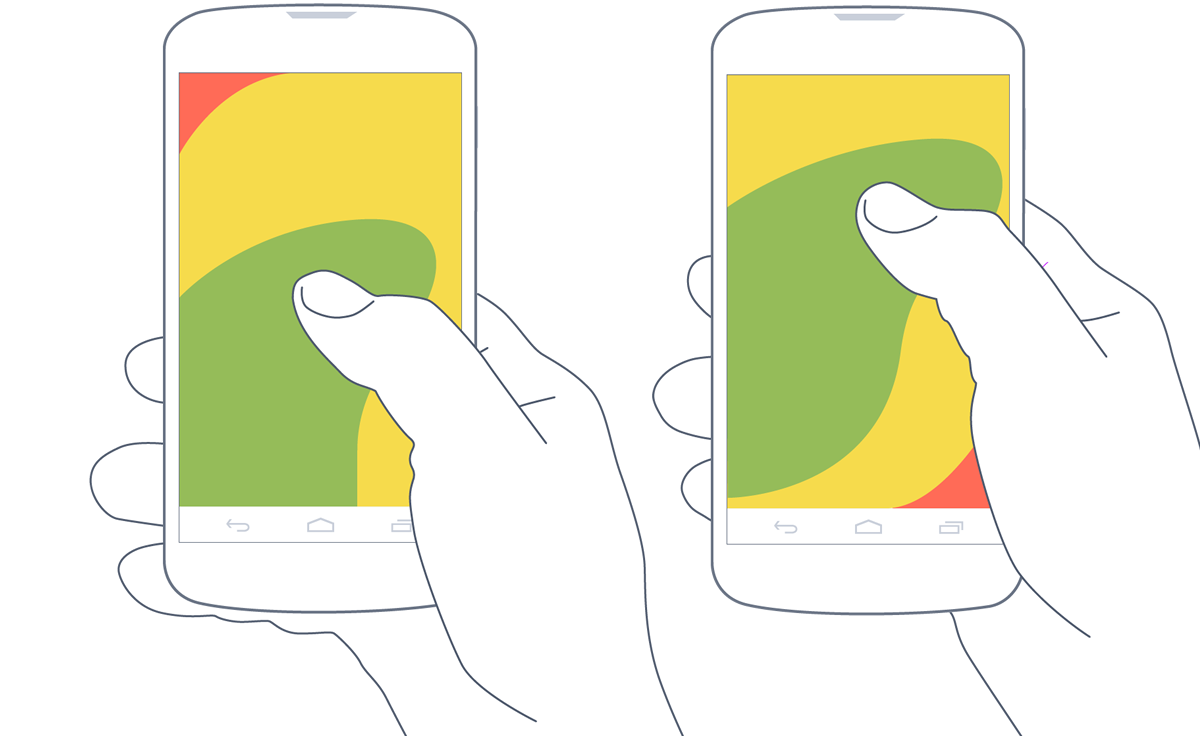
\includegraphics[height=6cm]{img/uso-movil.png}
\end{figure}

\end{frame}

%------------------------------------------------
\section{Patrones}
%------------------------------------------------
\subsection{Algunos patrones de diseño para dispositivos móviles}
%------------------------------------------------

\begin{frame}
\frametitle{Desborde de Acciones}

\begin{block}{En resumen:}
\justify
Las funciones extra y de uso poco frecuente se descubren por medio de la «\texttt{revelación progresiva}». Básicamente, están ocultas la mayor parte del tiempo, hasta que el usuario las reclame.
\end{block}

\begin{figure}[H]
  \centering
  
\includegraphics[height=3.5cm]{img/dots.jpg}
\end{figure}
\end{frame}

%------------------------------------------------

\begin{frame}
\frametitle{Desborde de Acciones}

\begin{columns}[c] % The "c" option specifies centered vertical alignment while the "t" option is used for top vertical alignment

\column{.5\textwidth} % Left column and width
\begin{block}{Android}
\justify
Las opciones que no caben en la barra de acción pasan automáticamente a mostrarse como acciones desbordadas. El camino para llegar a ellas es a través de un botón con un ícono de tres cuadrados verticales que las abre en formato de lista.
\end{block}

\column{.5\textwidth} % Right column and width
\begin{figure}[H]
  \centering
  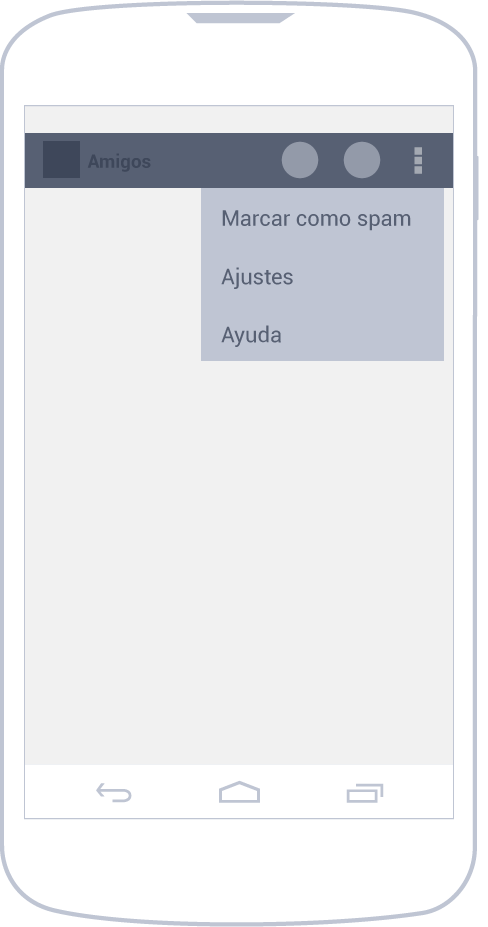
\includegraphics[height=6cm]{img/patron-acciones-desborde-01.png}
\end{figure}
\end{columns}
\end{frame}

%------------------------------------------------

\begin{frame}
\frametitle{Desborde de Acciones}

\begin{columns}[c] % The "c" option specifies centered vertical alignment while the "t" option is used for top vertical alignment

\column{.5\textwidth} % Left column and width
\begin{figure}[H]
  \centering
  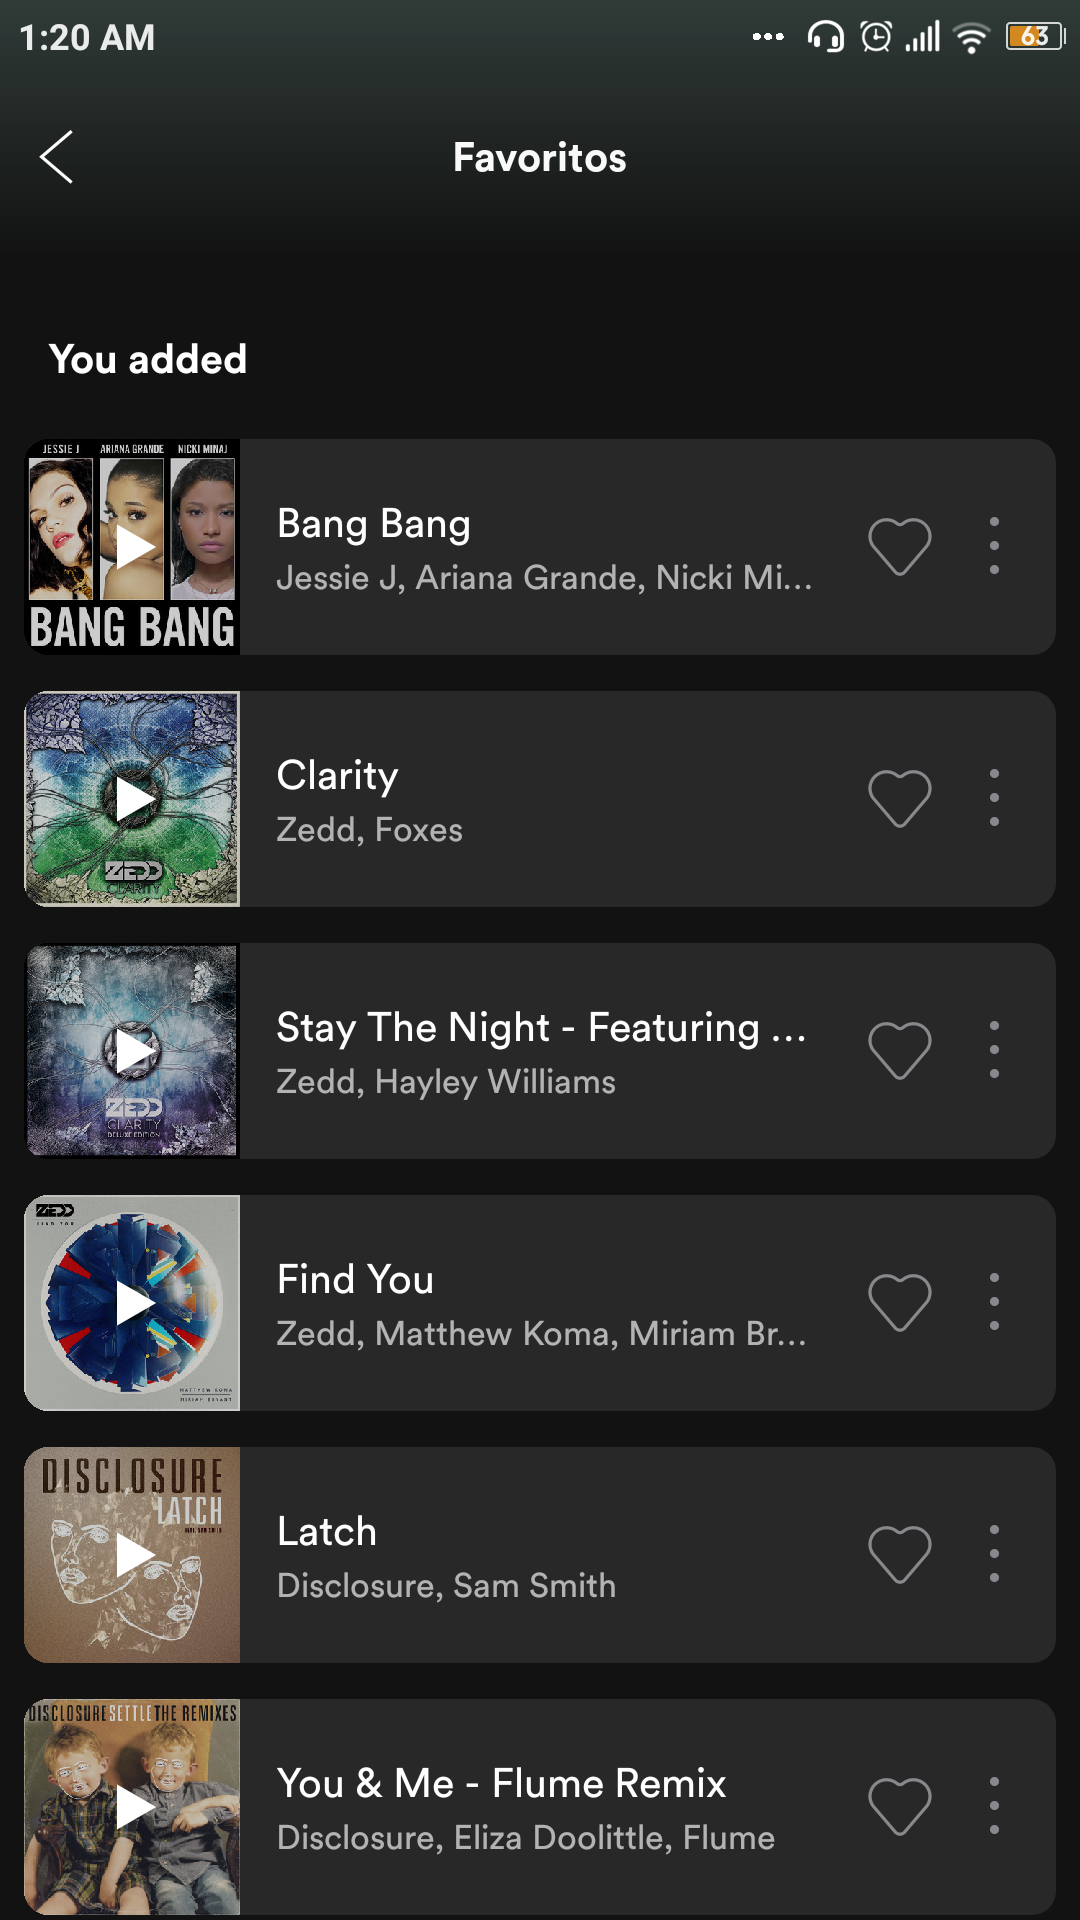
\includegraphics[height=6cm]{img/spotify-01.png}
\end{figure}

\column{.5\textwidth} % Right column and width
\begin{figure}[H]
  \centering
  
\includegraphics[height=6cm]{img/spotify-02.png}
\end{figure}

\end{columns}
\end{frame}

%------------------------------------------------

\begin{frame}
\frametitle{Desborde de Acciones}

\begin{columns}[c] % The "c" option specifies centered vertical alignment while the "t" option is used for top vertical alignment

\column{.5\textwidth} % Left column and width
\begin{figure}[H]
  \centering
  
\includegraphics[height=6cm]{img/spotify-03.png}
\end{figure}

\column{.5\textwidth} % Right column and width
\begin{figure}[H]
  \centering
  
\includegraphics[height=6cm]{img/spotify-04.png}
\end{figure}

\end{columns}
\end{frame}

%------------------------------------------------

\begin{frame}
\frametitle{Desborde de Acciones}

\begin{columns}[c] % The "c" option specifies centered vertical alignment while the "t" option is used for top vertical alignment

\column{.5\textwidth} % Left column and width
\begin{block}{iOS}
\justify
Consiste en agrupar acciones relacionadas, ocultas inicialmente, para luego mostrarlas en formato de lista de botones.
\end{block}

\column{.5\textwidth} % Right column and width
\begin{figure}[H]
  \centering
  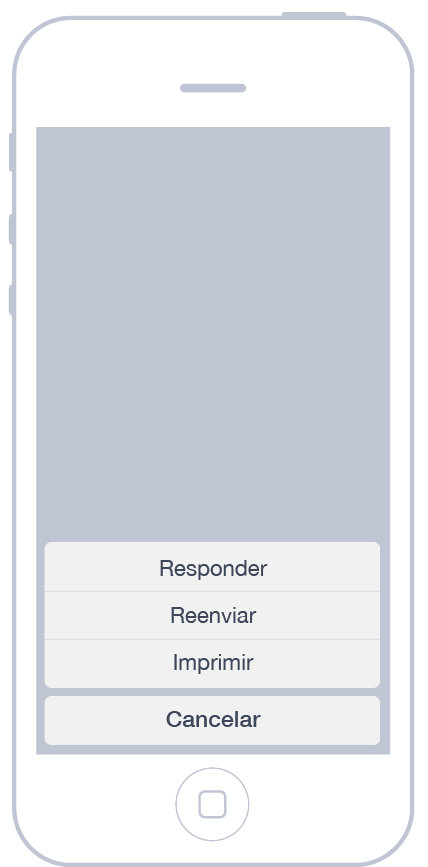
\includegraphics[height=6cm]{img/patron-acciones-desborde-02.png}
\end{figure}
\end{columns}
\end{frame}

%------------------------------------------------

\begin{frame}
\frametitle{Desborde de Acciones}

\begin{figure}[H]
  \centering
  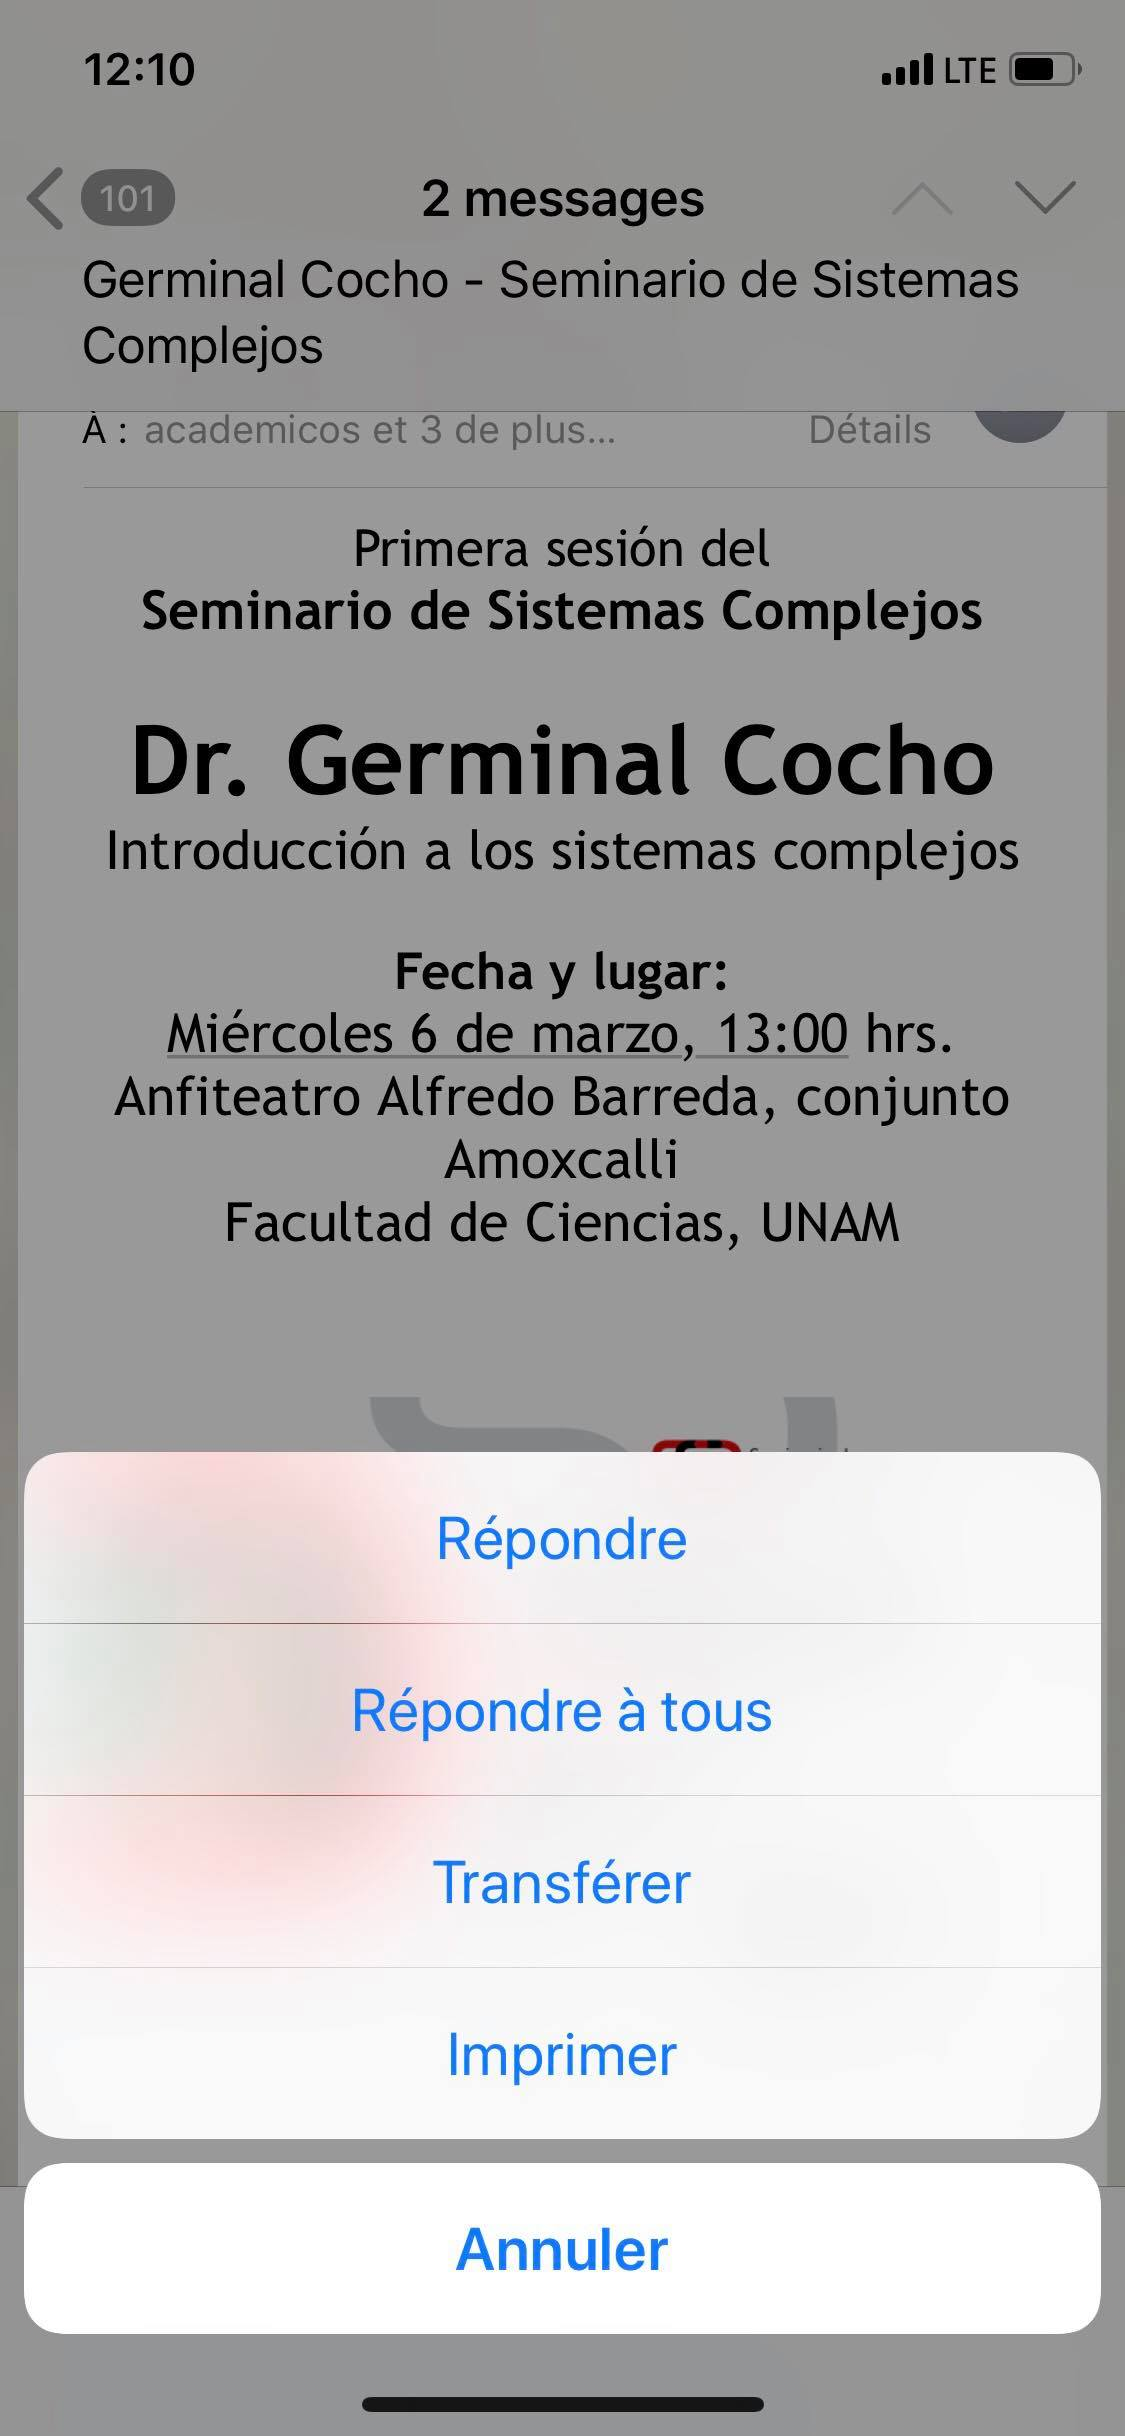
\includegraphics[height=6cm]{img/mail-01.jpg}
\end{figure}
\end{frame}


%------------------------------------------------

\begin{frame}
\frametitle{Desborde de Acciones}

\begin{columns}[c] % The "c" option specifies centered vertical alignment while the "t" option is used for top vertical alignment

\column{.5\textwidth} % Left column and width
\begin{block}{Windows Phone}
\justify
Al igual que Android, las acciones extra se ubican por debajo de la barra de acción y se indican con puntos suspensivos que, al pulsarlos, despliegan las acciones ocultas en formato de lista.
\end{block}

\column{.5\textwidth} % Right column and width
\begin{figure}[H]
  \centering
  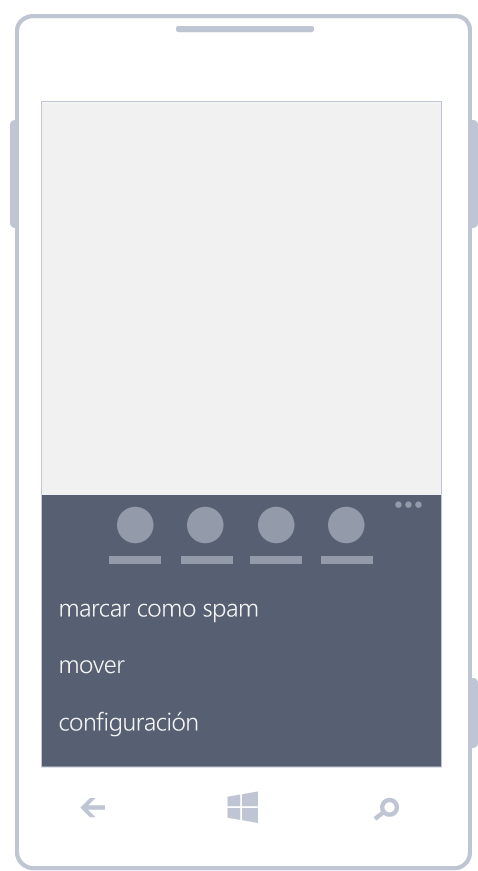
\includegraphics[height=6cm]{img/patron-acciones-desborde-03.png}
\end{figure}
\end{columns}
\end{frame}

%------------------------------------------------

\begin{frame}
\frametitle{Accesos Rápidos}

\begin{block}{En resumen:}
\justify
Hay ciertas acciones que deben estar muy a mano para que los usuarios puedan alcanzar sus objetivos rápidamente, por ejemplo, acceder a las acciones asociadas a ítems en una lista o retícula sin tener que navegar en profundidad para encontrarlas.
\end{block}

\begin{figure}[H]
  \centering
  
\includegraphics[height=3cm]{img/quick.png}
\end{figure}
\end{frame}

%------------------------------------------------

\begin{frame}
\frametitle{Accesos Rápidos}

\begin{columns}[c] % The "c" option specifies centered vertical alignment while the "t" option is used for top vertical alignment

\column{.5\textwidth} % Left column and width
\begin{block}{Android}
\justify
Para llegar a las acciones rápidas es posible mediante un ícono triangular ubicado al pie de los elementos que tienen este tipo de acciones asociadas.
\end{block}

\column{.5\textwidth} % Right column and width
\begin{figure}[H]
  \centering
  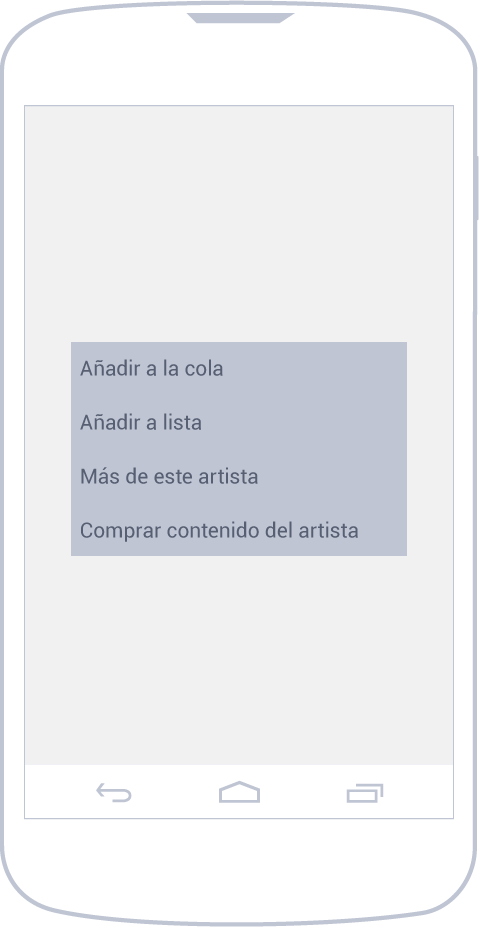
\includegraphics[height=6cm]{img/patron-accesos-rapidos-01.png}
\end{figure}
\end{columns}
\end{frame}

%------------------------------------------------

\begin{frame}
\frametitle{Accesos Rápidos}

\begin{columns}[c] % The "c" option specifies centered vertical alignment while the "t" option is used for top vertical alignment

\column{.5\textwidth} % Left column and width
\begin{figure}[H]
  \centering
  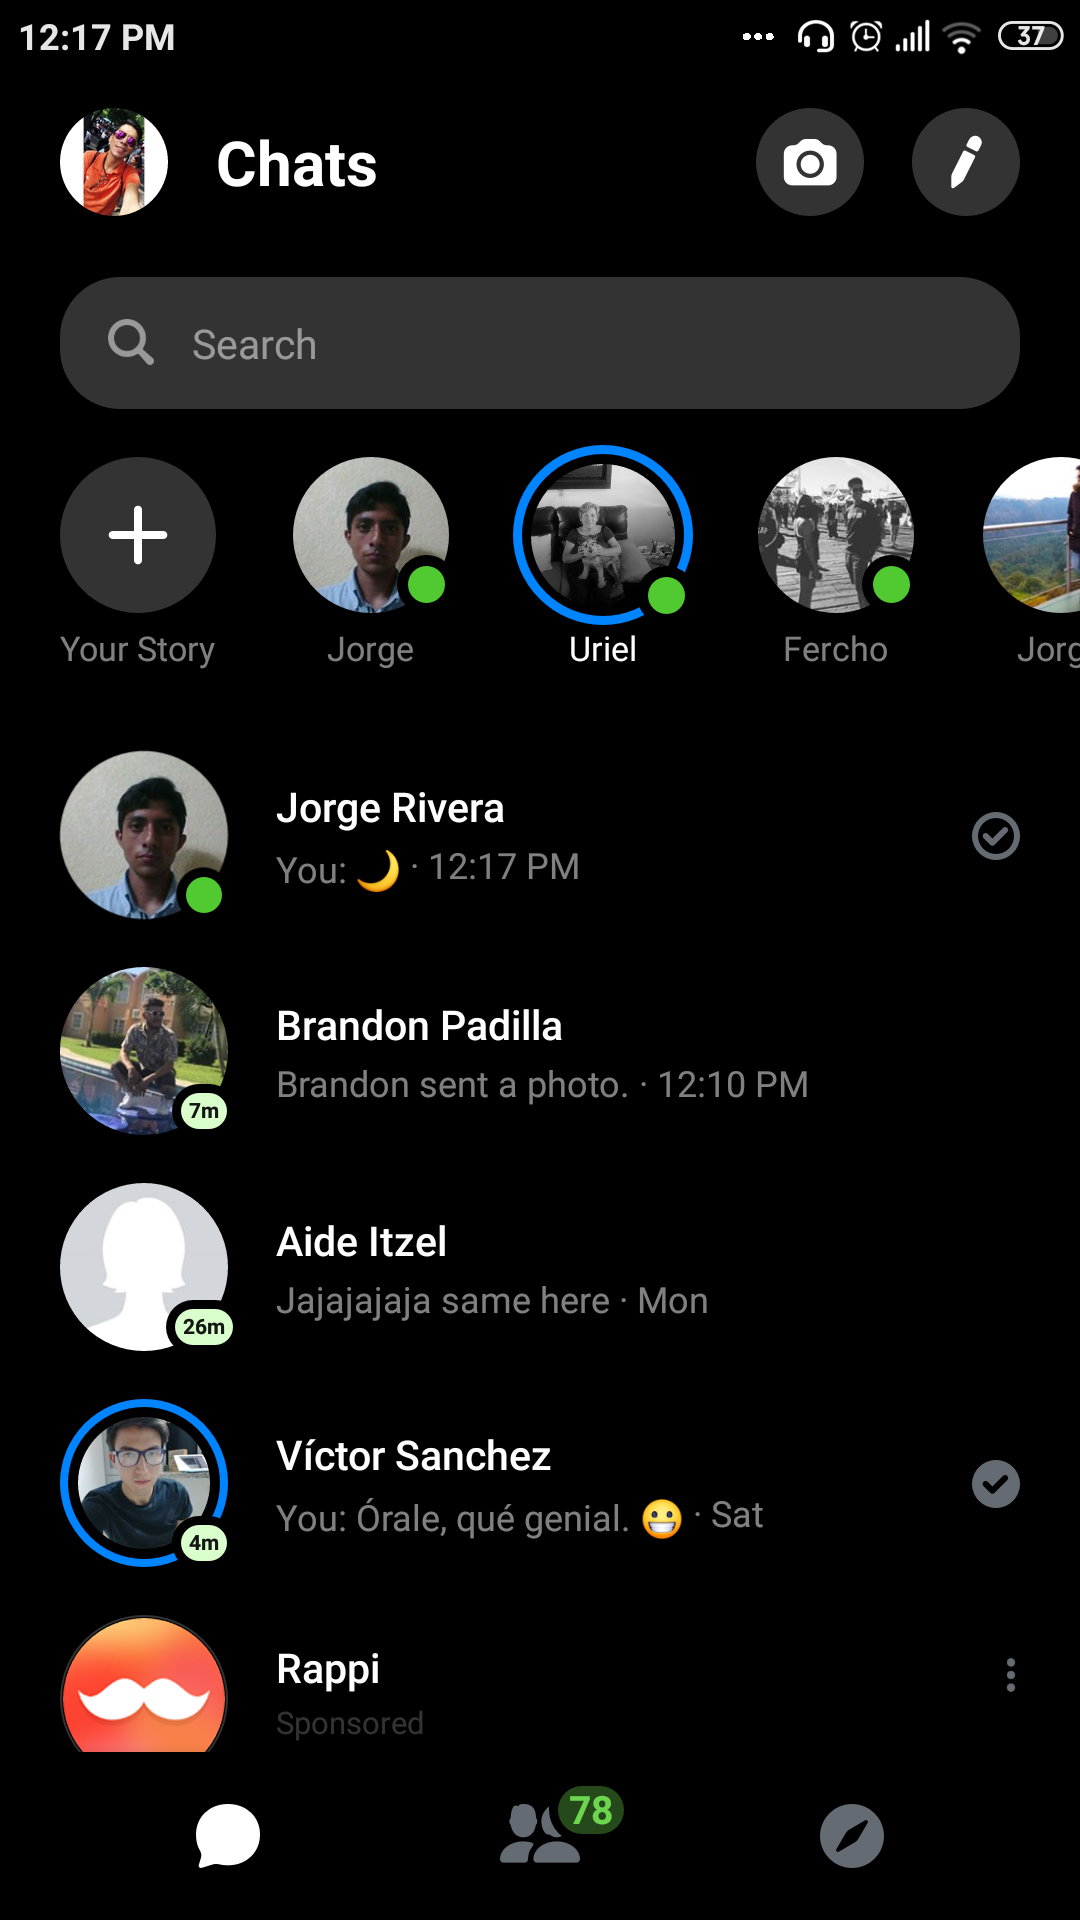
\includegraphics[height=6cm]{img/facebook-01.png}
\end{figure}

\column{.5\textwidth} % Right column and width
\begin{figure}[H]
  \centering
  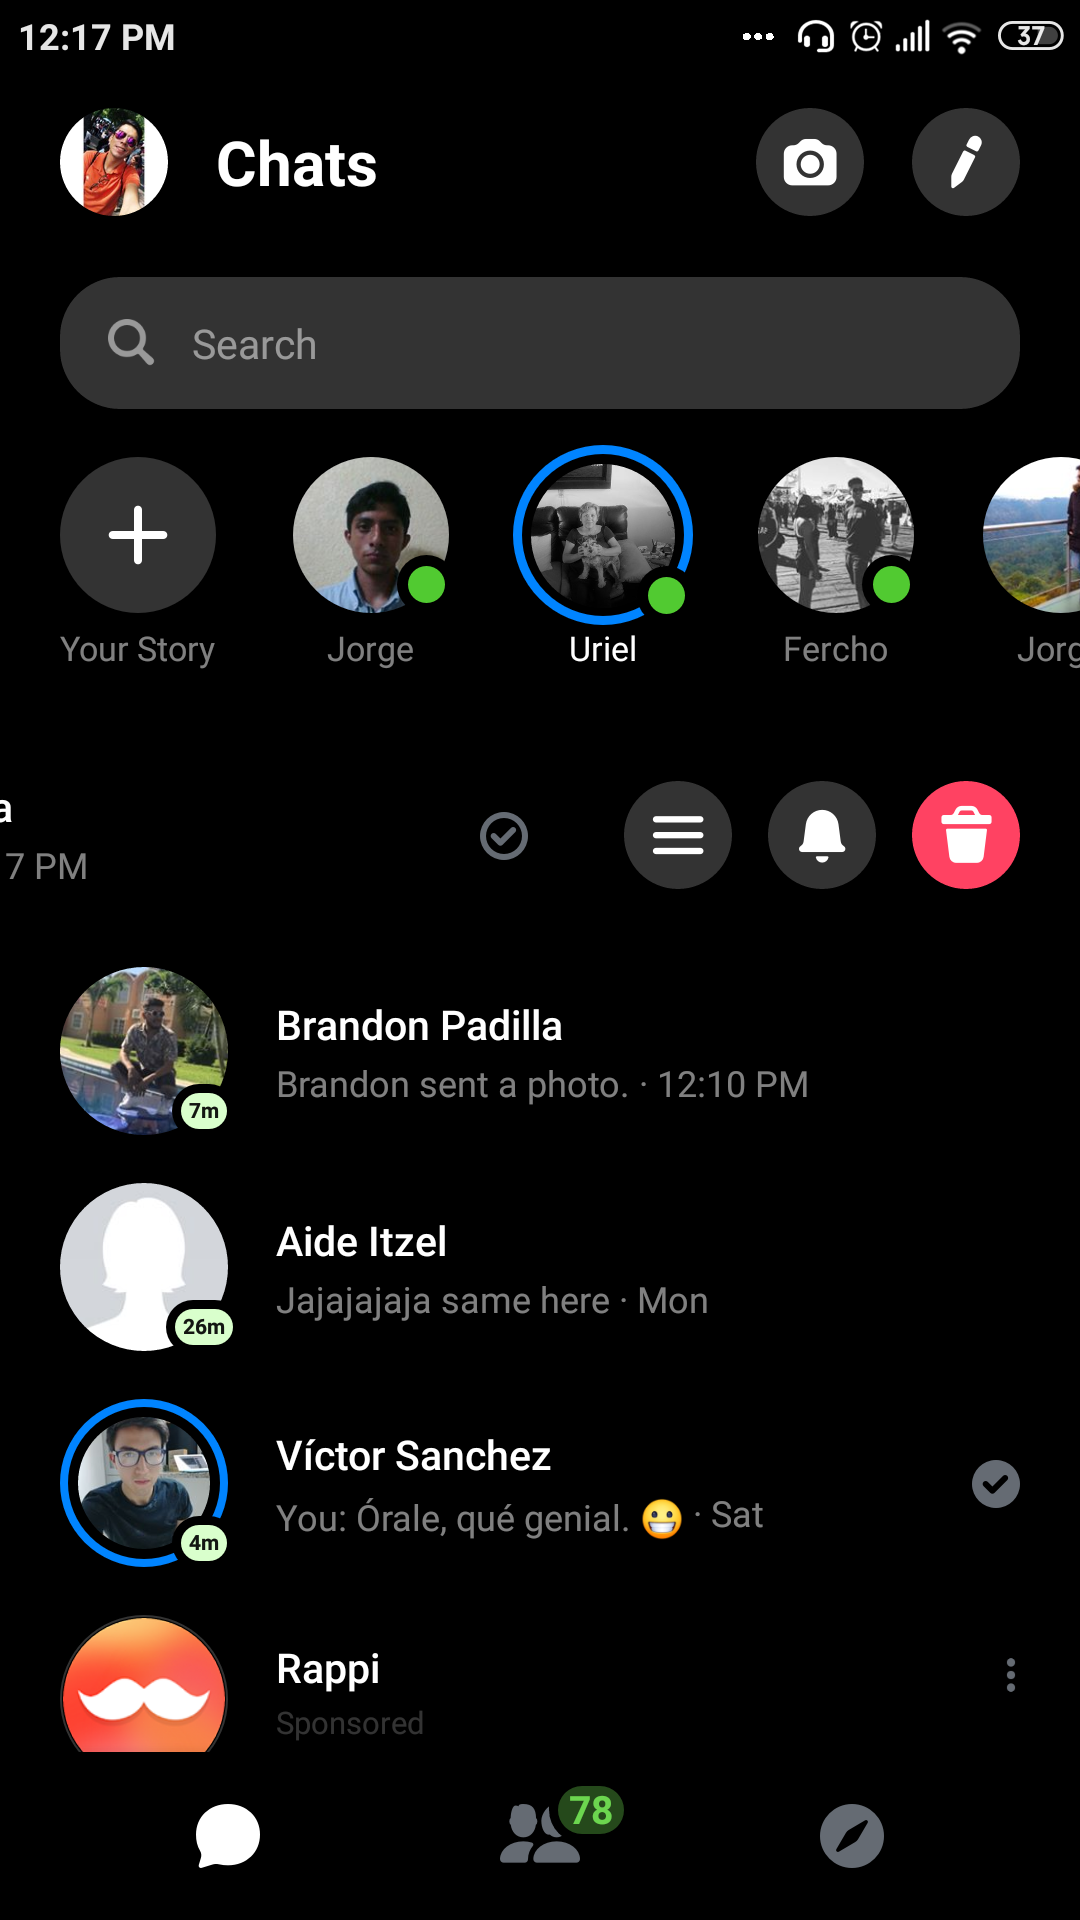
\includegraphics[height=6cm]{img/facebook-02.png}
\end{figure}

\end{columns}
\end{frame}

%------------------------------------------------

\begin{frame}
\frametitle{Accesos Rápidos}

\begin{columns}[c] % The "c" option specifies centered vertical alignment while the "t" option is used for top vertical alignment

\column{.5\textwidth} % Left column and width
\begin{block}{iOS}
\justify
Un ejemplo bastante común de acceso rápido es en este sistema operativo, es cuando se quiere eliminar un ítem de una lista y se realiza un deslizamiento horizontal sobre la fila deseada. Por otro lado, las acciones relacionadas se ubican \textit{in situ}, sobre el mismo ítem.
\end{block}

\column{.5\textwidth} % Right column and width
\begin{figure}[H]
  \centering
  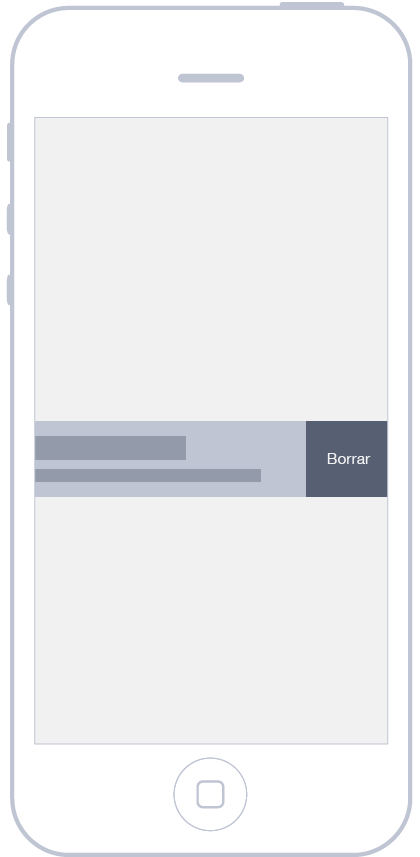
\includegraphics[height=6cm]{img/patron-accesos-rapidos-02.png}
\end{figure}
\end{columns}

\end{frame}
%------------------------------------------------

\begin{frame}
\frametitle{Accesos Rápidos}

\begin{figure}[H]
  \centering
  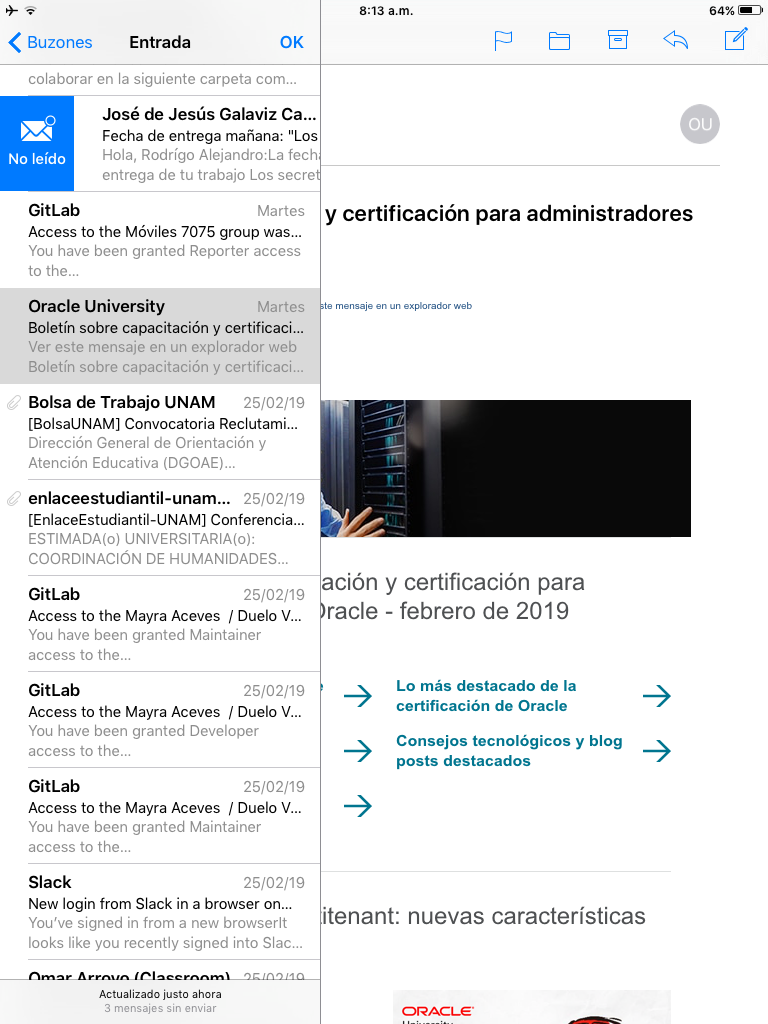
\includegraphics[height=6cm]{img/correo-01.PNG}
\end{figure}

\end{frame}

%------------------------------------------------

\begin{frame}
\frametitle{Accesos Rápidos}

\begin{columns}[c] % The "c" option specifies centered vertical alignment while the "t" option is used for top vertical alignment

\column{.5\textwidth} % Left column and width
\begin{block}{Windows Phone}
\justify
Se despliegan en formato de menú contextual al efectuar el gesto de mantener pulsado sobre un ítem.
\end{block}

\column{.5\textwidth} % Right column and width
\begin{figure}[H]
  \centering
  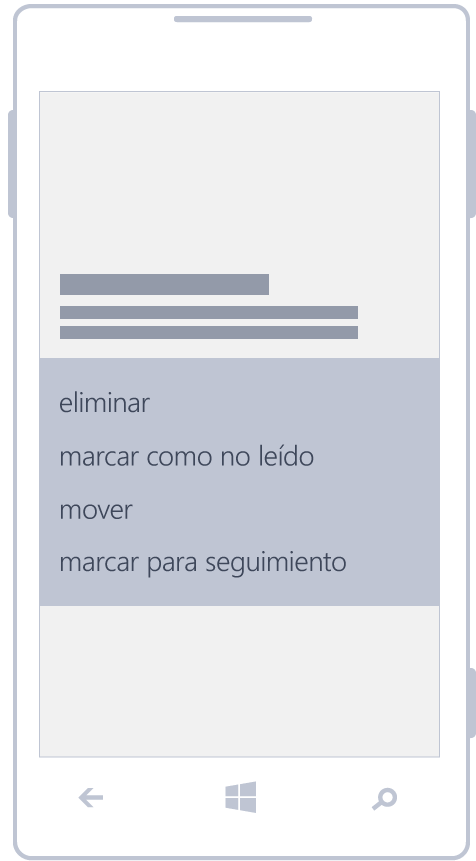
\includegraphics[height=6cm]{img/patron-accesos-rapidos-03.png}
\end{figure}
\end{columns}
\end{frame}

%------------------------------------------------

\begin{frame}
\frametitle{Buscar}

\begin{block}{En resumen:}
\justify
Teniendo en cuenta que uno de los usos principales del móvil es el consumo de contenidos, la herramienta «buscar» es una manera esencial de llegar a ellos. En apps que muestran grandes cantidades de datos, la búsqueda puede ser incluso la función primaria.
\end{block}

\begin{figure}[H]
  \centering
  
\includegraphics[height=3.5cm]{img/magnifying-glass.png}
\end{figure}
\end{frame}

%------------------------------------------------

\begin{frame}
\frametitle{Buscar}

\begin{columns}[c] % The "c" option specifies centered vertical alignment while the "t" option is used for top vertical alignment

\column{.5\textwidth} % Left column and width
\begin{block}{Android}
\justify
Aquí la opción para buscar sea accesible desde la barra de acciones. Si la búsqueda es una característica importante para la aplicación, debería ocupar la primera posición de esta barra. Al pulsar «\texttt{buscar}», la barra superior se modifica para convertirse en la de búsqueda.
\end{block}

\column{.5\textwidth} % Right column and width
\begin{figure}[H]
  \centering
  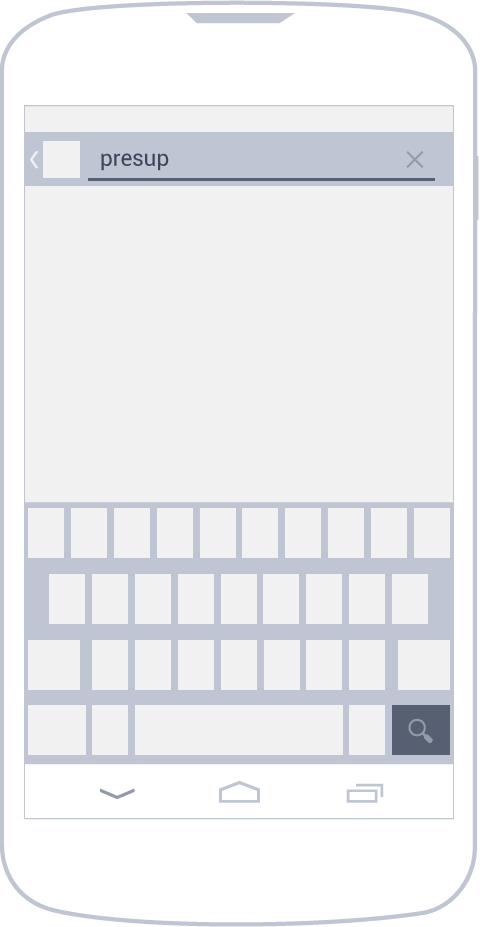
\includegraphics[height=6cm]{img/patron-buscar-01.png}
\end{figure}
\end{columns}
\end{frame}

%------------------------------------------------

\begin{frame}
\frametitle{Buscar}

\begin{columns}[c] % The "c" option specifies centered vertical alignment while the "t" option is used for top vertical alignment

\column{.5\textwidth} % Left column and width
\begin{figure}[H]
  \centering
  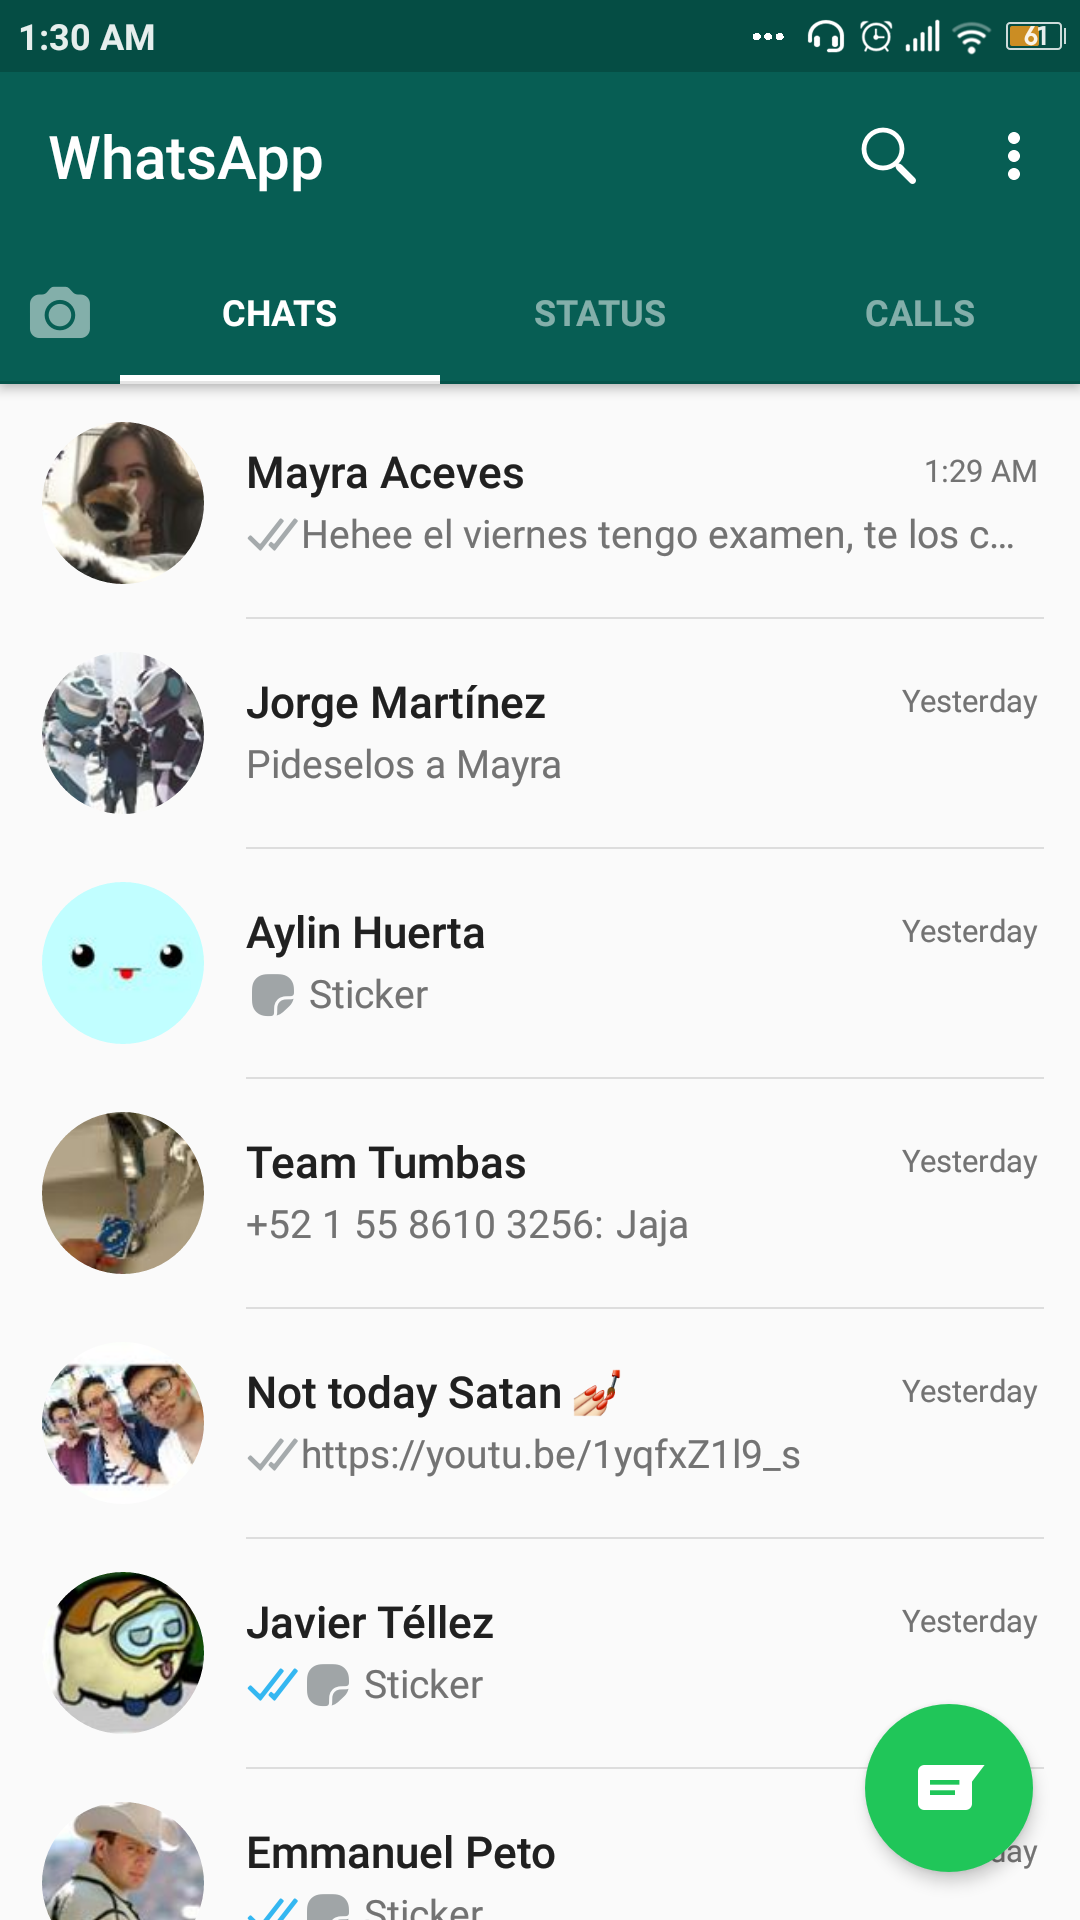
\includegraphics[height=6cm]{img/whatsapp-01.png}
\end{figure}

\column{.5\textwidth} % Right column and width
\begin{figure}[H]
  \centering
  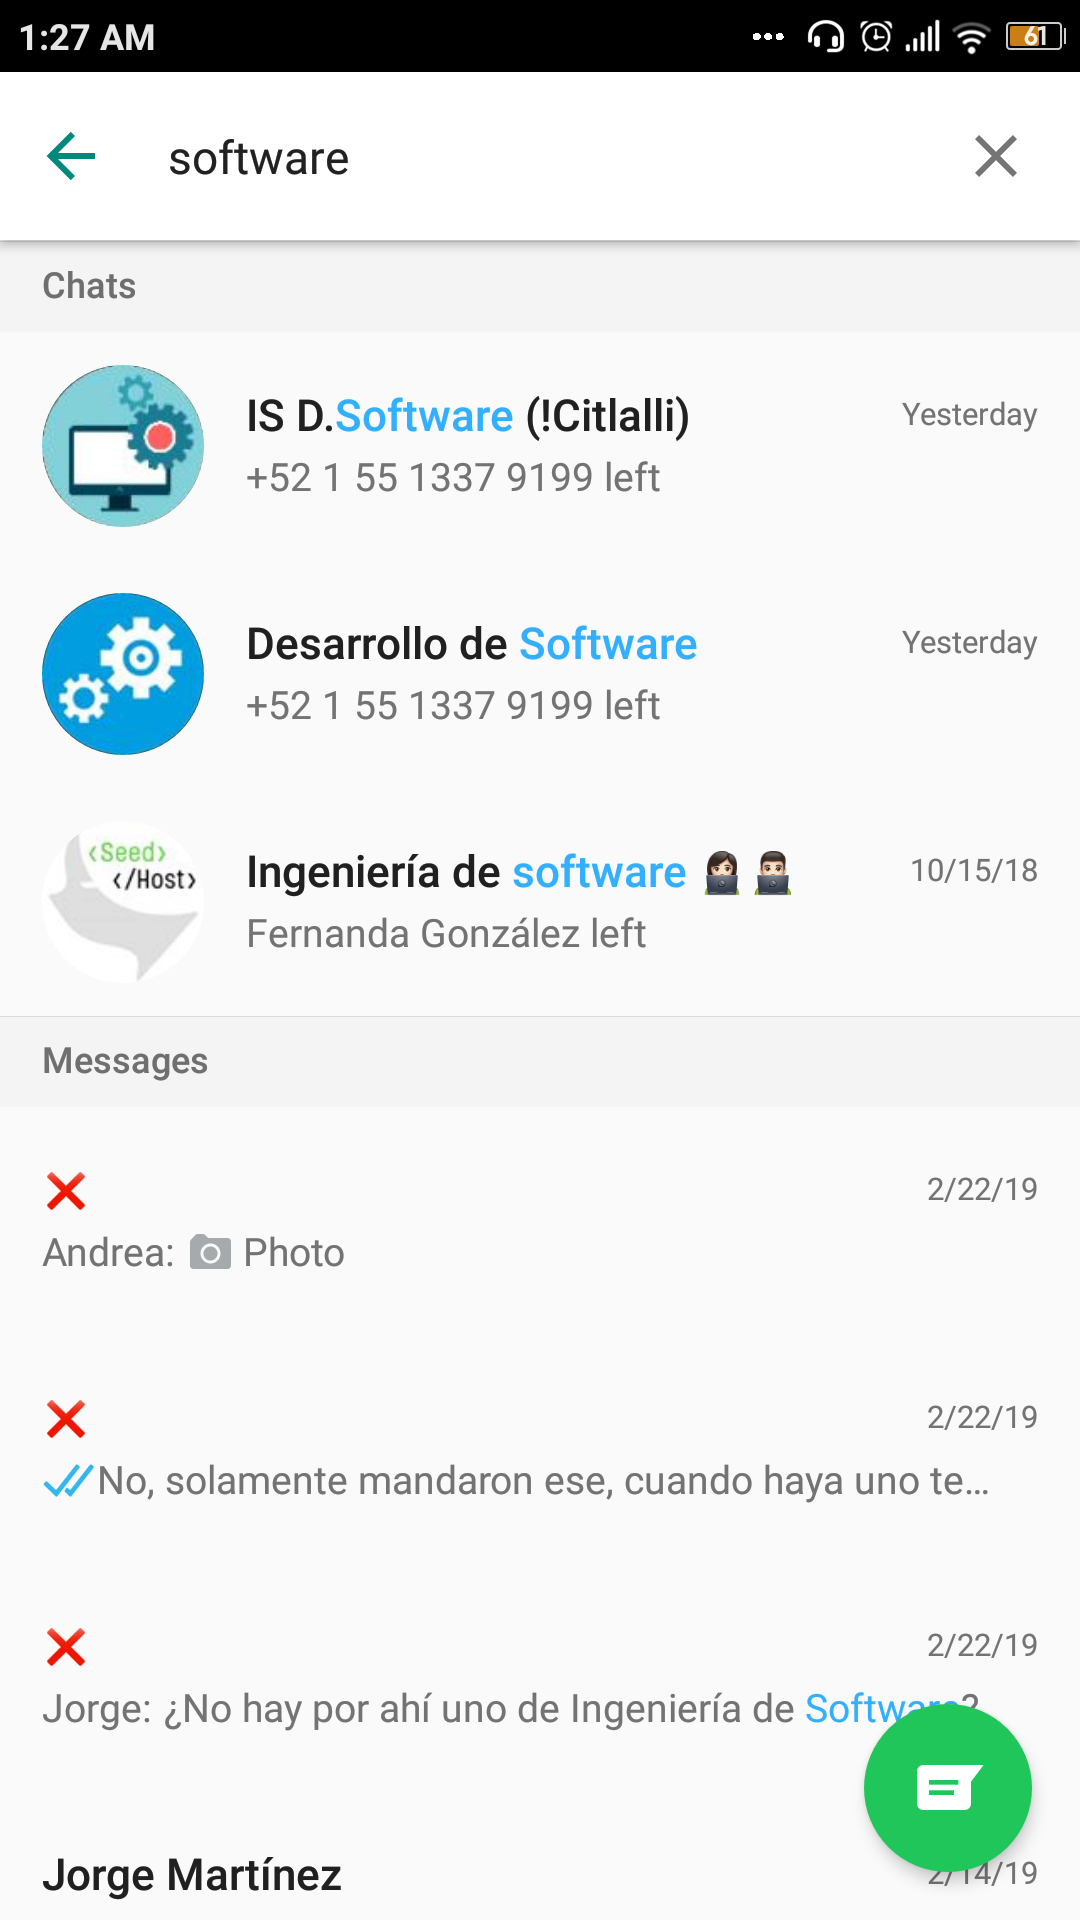
\includegraphics[height=6cm]{img/whatsapp-02.png}
\end{figure}

\end{columns}
\end{frame}

%------------------------------------------------

\begin{frame}
\frametitle{Buscar}

\begin{columns}[c] % The "c" option specifies centered vertical alignment while the "t" option is used for top vertical alignment

\column{.5\textwidth} % Left column and width
\begin{block}{iOS}
\justify
En iPhone es habitual encontrar un campo de búsqueda por encima de las listas, tal como aparece en \textit{Contactos} y otras apps. Junto con el campo de texto pueden aparecer filtros para refinar las búsquedas más complejas.
\end{block}

\column{.5\textwidth} % Right column and width
\begin{figure}[H]
  \centering
  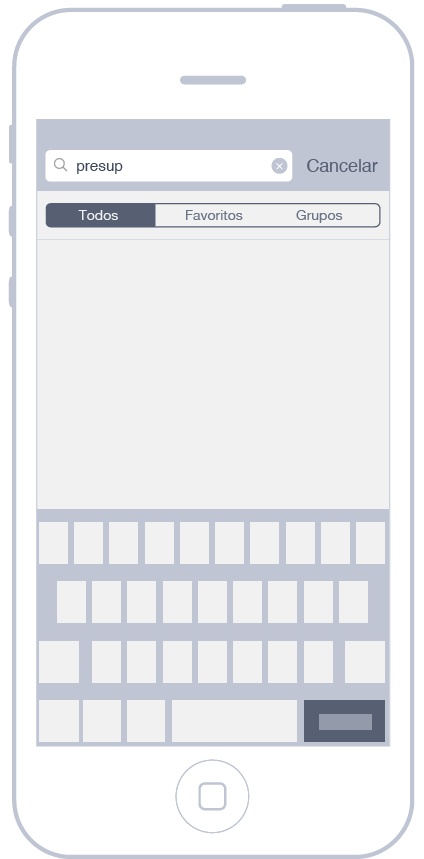
\includegraphics[height=6cm]{img/patron-buscar-02.png}
\end{figure}
\end{columns}
\end{frame}

%------------------------------------------------

\begin{frame}
\frametitle{Buscar}

\begin{columns}[c] % The "c" option specifies centered vertical alignment while the "t" option is used for top vertical alignment

\column{.5\textwidth} % Left column and width
\begin{figure}[H]
  \centering
  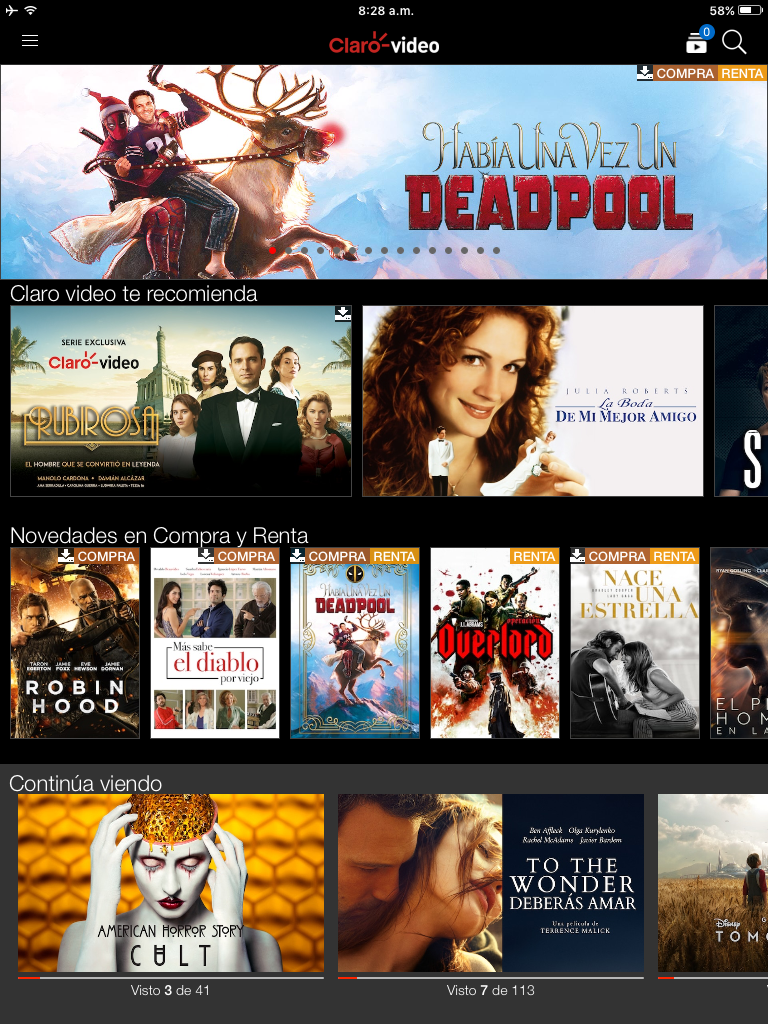
\includegraphics[height=6cm]{img/clarovideo-01.PNG}
\end{figure}

\column{.5\textwidth} % Right column and width
\begin{figure}[H]
  \centering
  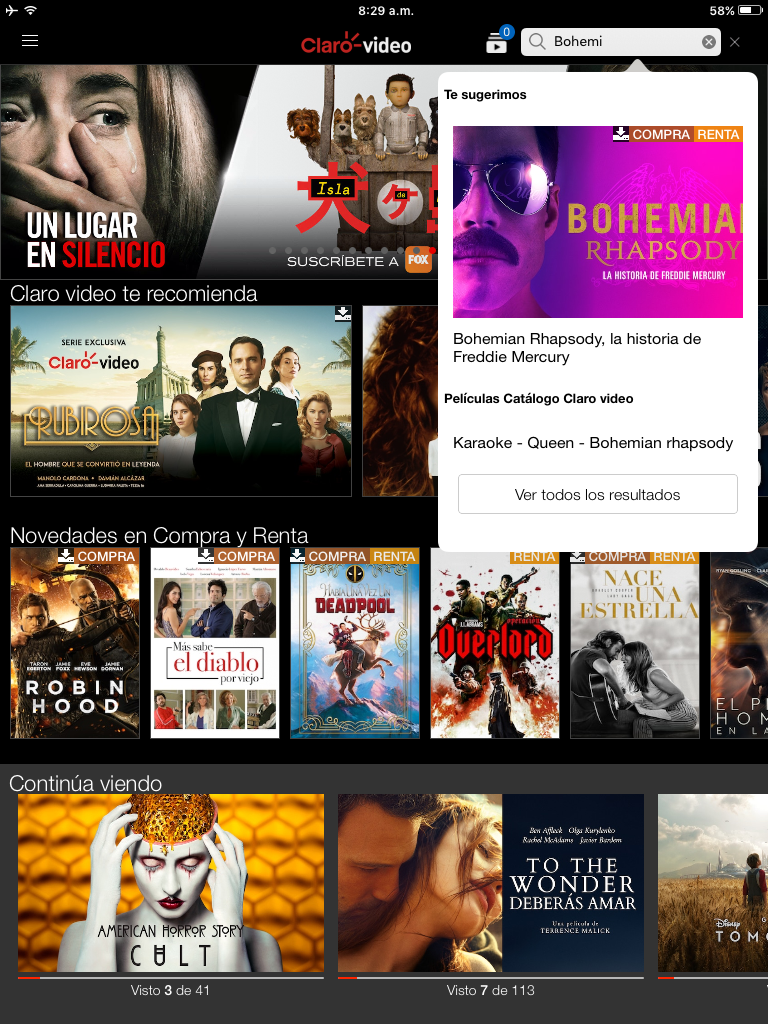
\includegraphics[height=6cm]{img/clarovideo-02.PNG}
\end{figure}

\end{columns}
\end{frame}

%------------------------------------------------

\begin{frame}
\frametitle{Buscar}

\begin{columns}[c] % The "c" option specifies centered vertical alignment while the "t" option is used for top vertical alignment

\column{.5\textwidth} % Left column and width
\begin{block}{Windows Phone}
\justify
La búsqueda es tratada como una acción más, disponible en la barra de acciones y se lleva a cabo en una página separada, donde se introduce el texto y se listan los resultados.
\end{block}

\column{.5\textwidth} % Right column and width
\begin{figure}[H]
  \centering
  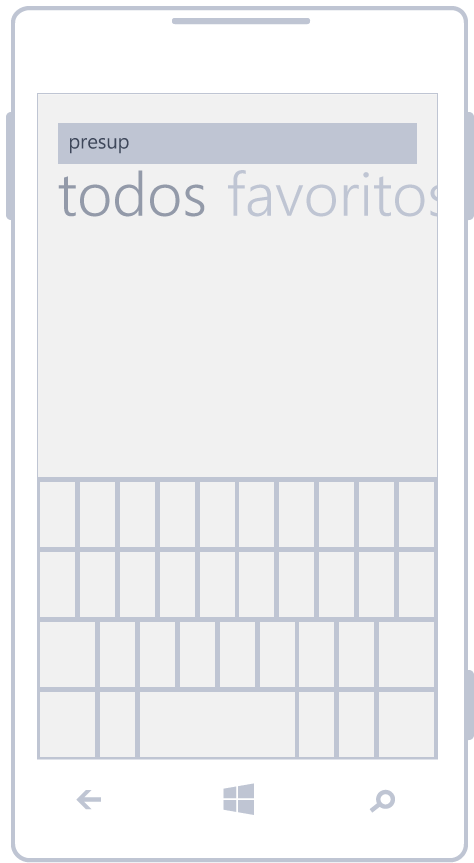
\includegraphics[height=6cm]{img/patron-buscar-03.png}
\end{figure}
\end{columns}
\end{frame}

%------------------------------------------------

\begin{frame}
\frametitle{Edición de Listas}

\begin{block}{En resumen:}
\justify
Es posible que el usuario necesite modificar varios elementos de una lista de forma simultánea. El flujo para realizarlo es bastante sencillo: se seleccionan los elementos sobre los que se quiere actuar y luego se aplica la acción correspondiente.
\end{block}
\begin{figure}[H]
  \centering
  
\includegraphics[height=3.5cm]{img/list.png}
\end{figure}
\end{frame}

%------------------------------------------------

\begin{frame}
\frametitle{Edición de Listas}

\begin{columns}[c] % The "c" option specifies centered vertical alignment while the "t" option is used for top vertical alignment

\column{.5\textwidth} % Left column and width
\begin{block}{Android}
\justify
La selección múltiple se realiza manteniendo pulsado un elemento. Una vez seleccionado el primer ítem, la barra de acción cambia indicando cuántos elementos están seleccionados y qué acciones se pueden realizar. Para salir de esta vista, Android propone hacerlo con el botón «\texttt{check}».
\end{block}

\column{.5\textwidth} % Right column and width
\begin{figure}[H]
  \centering
  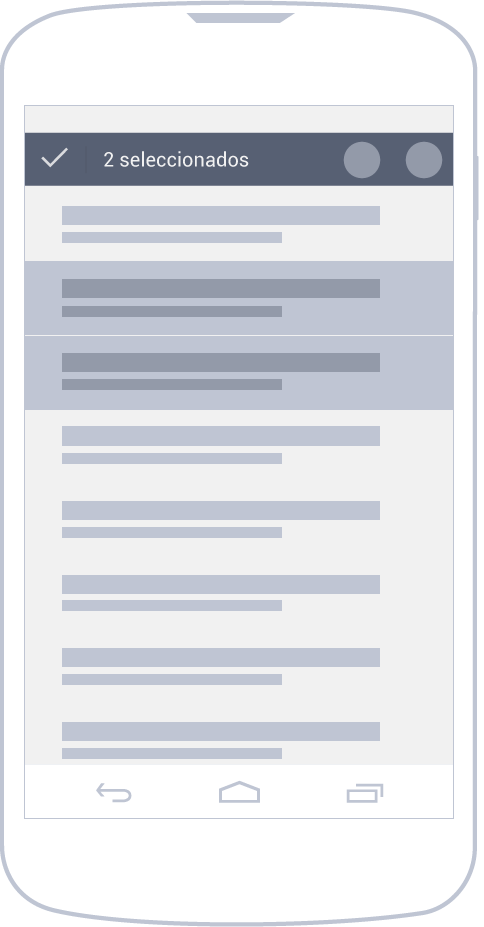
\includegraphics[height=6cm]{img/patron-acciones-masivas-01.png}
\end{figure}
\end{columns}
\end{frame}

%------------------------------------------------

\begin{frame}
\frametitle{Edición de Listas}

\begin{columns}[c] % The "c" option specifies centered vertical alignment while the "t" option is used for top vertical alignment

\column{.5\textwidth} % Left column and width
\begin{figure}[H]
  \centering
  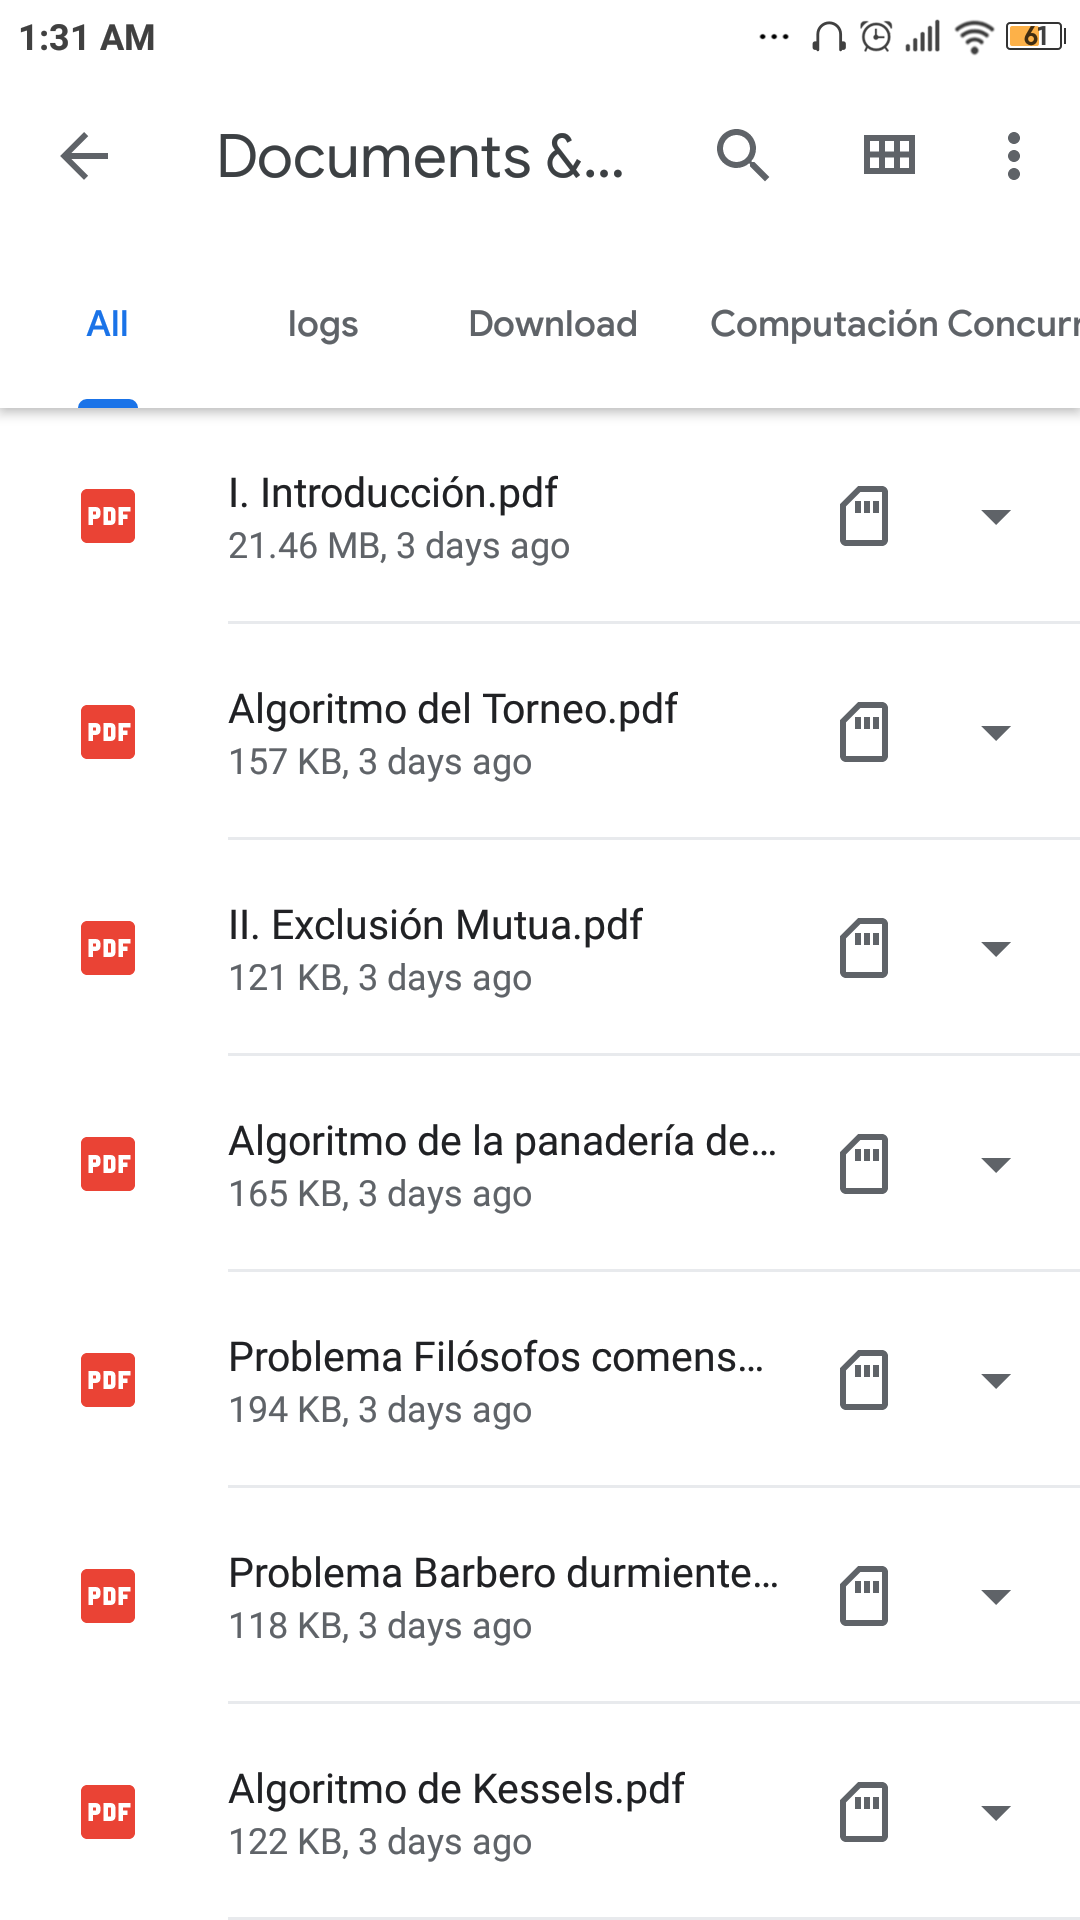
\includegraphics[height=6cm]{img/google-files-01.png}
\end{figure}

\column{.5\textwidth} % Right column and width
\begin{figure}[H]
  \centering
  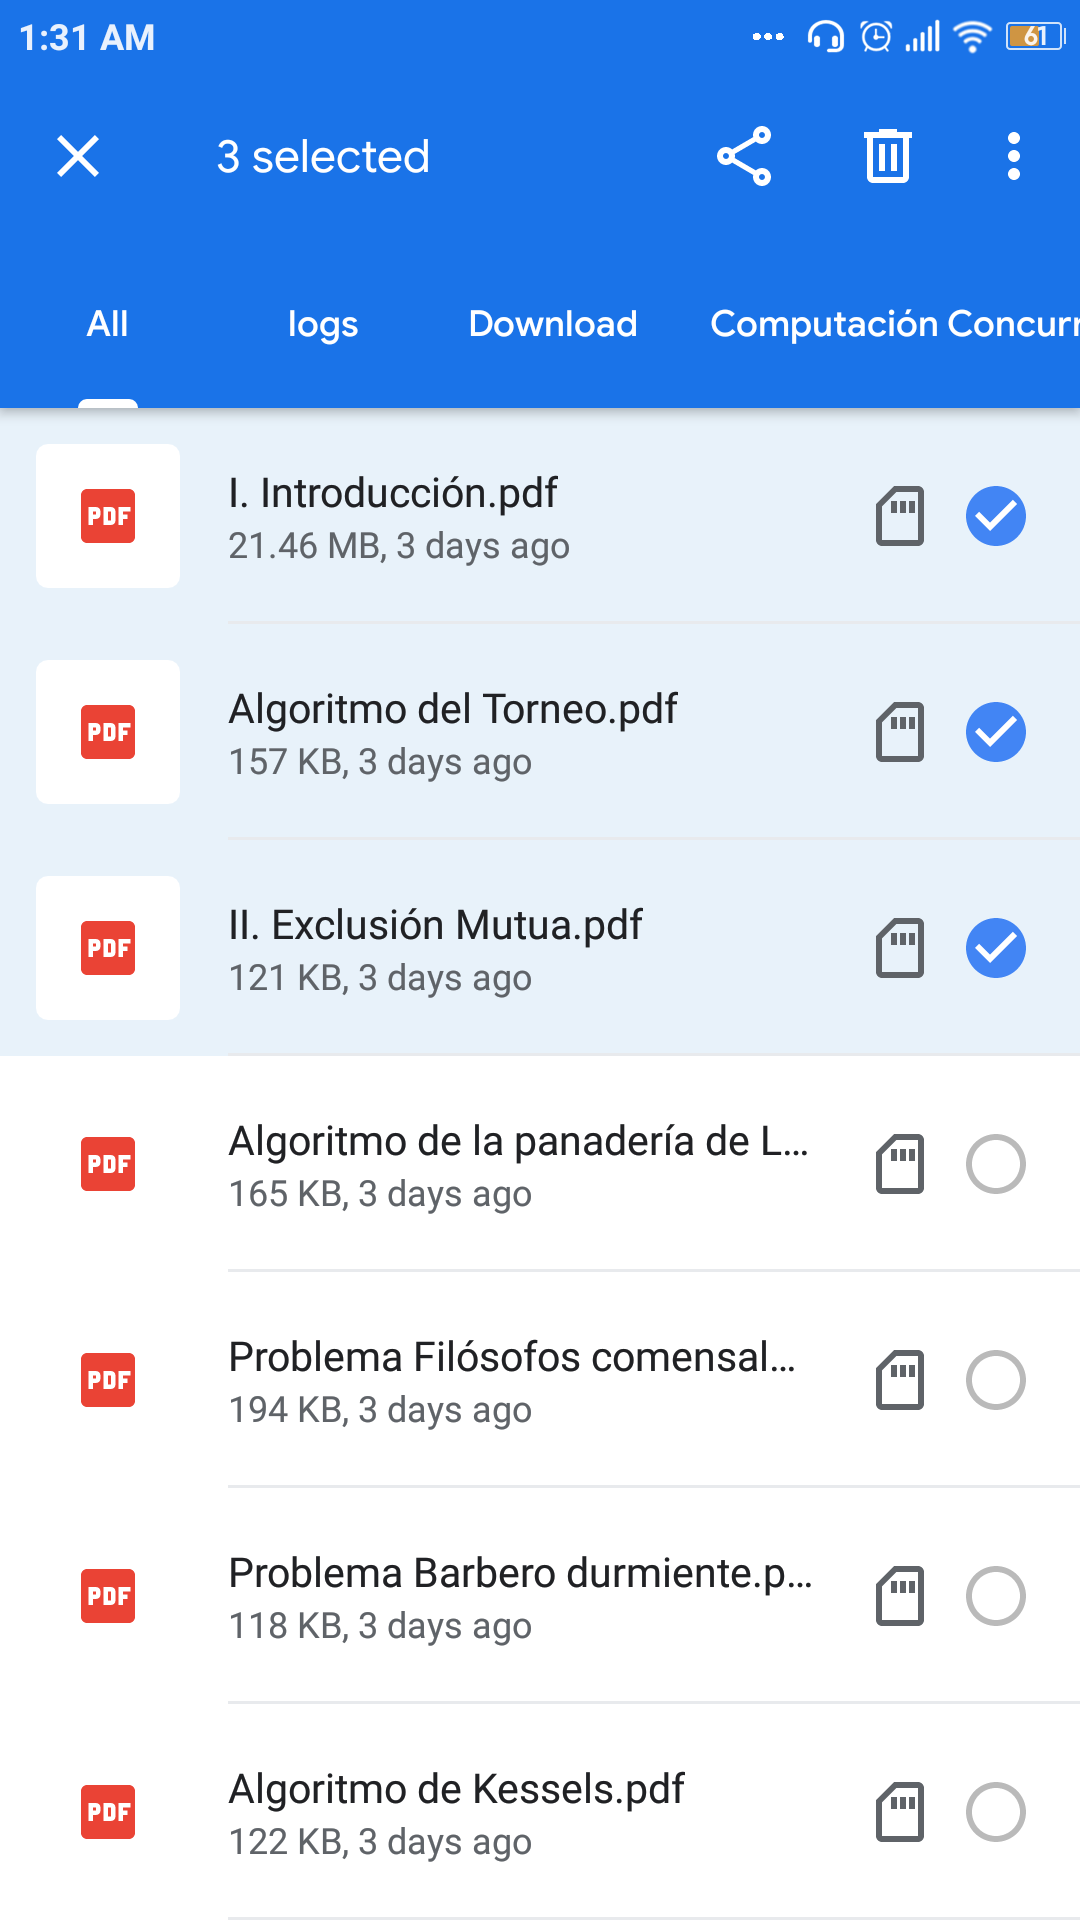
\includegraphics[height=6cm]{img/google-files-02.png}
\end{figure}

\end{columns}
\end{frame}

%------------------------------------------------

\begin{frame}
\frametitle{Edición de Listas}

\begin{columns}[c] % The "c" option specifies centered vertical alignment while the "t" option is used for top vertical alignment

\column{.5\textwidth} % Left column and width
\begin{block}{iOS}
\justify
La edición de listas suele activarse por medio de un botón «\texttt{editar}» colocado en la barra superior. De esta forma, la selección se hace visible junto con las acciones relacionadas. Para salir de esta vista sin aplicar los cambios, en el mismo sitio por donde se ha accedido, ahora hay un «\texttt{cancelar}».
\end{block}

\column{.5\textwidth} % Right column and width
\begin{figure}[H]
  \centering
  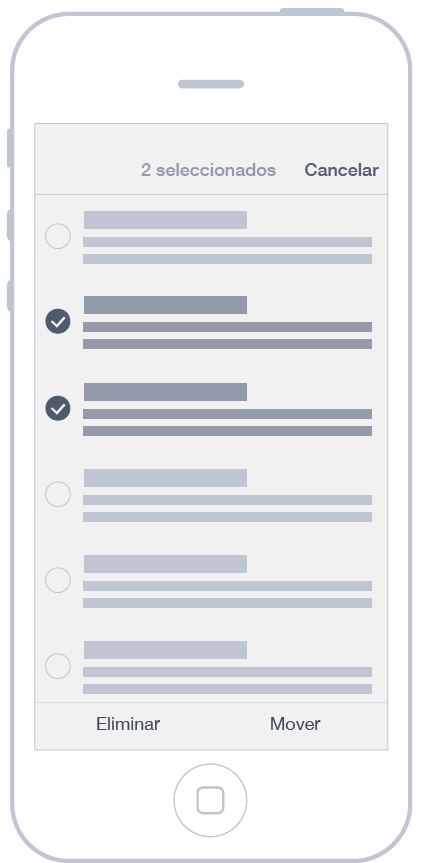
\includegraphics[height=6cm]{img/patron-acciones-masivas-02.png}
\end{figure}
\end{columns}
\end{frame}

%------------------------------------------------

\begin{frame}
\frametitle{Edición de Listas}

\begin{columns}[c] % The "c" option specifies centered vertical alignment while the "t" option is used for top vertical alignment

\column{.5\textwidth} % Left column and width
\begin{figure}[H]
  \centering
  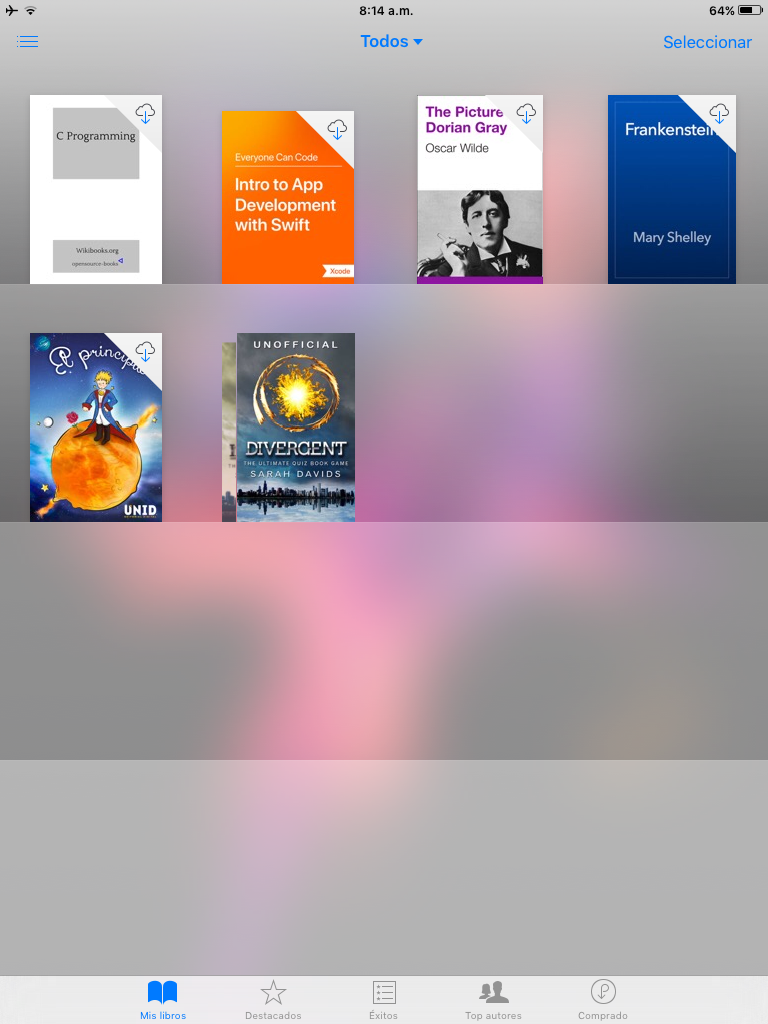
\includegraphics[height=6cm]{img/books-01.PNG}
\end{figure}

\column{.5\textwidth} % Right column and width
\begin{figure}[H]
  \centering
  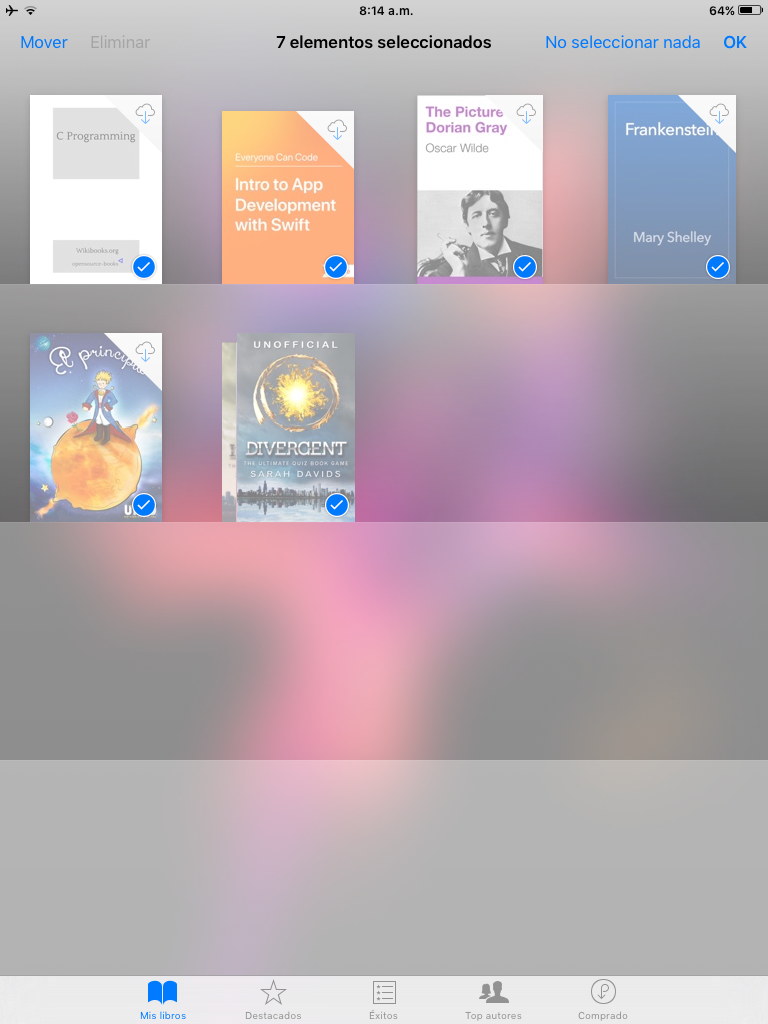
\includegraphics[height=6cm]{img/books-02.PNG}
\end{figure}

\end{columns}
\end{frame}

%------------------------------------------------

\begin{frame}
\frametitle{Edición de Listas}

\begin{columns}[c] % The "c" option specifies centered vertical alignment while the "t" option is used for top vertical alignment

\column{.5\textwidth} % Left column and width
\begin{block}{Windows Phone}
\justify
A través de la barra de acciones donde el usuario encuentra la opción «\texttt{seleccionar}» o usando un atajo que resulta muy práctico una vez aprendido: el truco está en tocar el primer ítem en su lateral izquierdo. De esta forma se hace visible la lista en el modo de edición, lo que permite seleccionar varios ítems a la vez.
\end{block}

\column{.5\textwidth} % Right column and width
\begin{figure}[H]
  \centering
  
\includegraphics[height=6cm]{img/patron-acciones-masivas-03.png}
\end{figure}
\end{columns}
\end{frame}

%------------------------------------------------

\begin{frame}
\frametitle{Cuadro de Diálogos}

\begin{block}{En resumen:}
\justify
Hay casos puntuales en los que hay que interrumpir al usuario de forma temporal para que tome una decisión o para explicarle mejor algo que ha sucedido antes de continuar una tarea. Con los diálogos visibles en pantalla no es posible hacer otra cosa en la aplicación.
\end{block}

\begin{figure}[H]
  \centering
  
\includegraphics[height=3cm]{img/notification.png}
\end{figure}
\end{frame}

%------------------------------------------------

\begin{frame}
\frametitle{Cuadro de Diálogos}

\begin{columns}[c] % The "c" option specifies centered vertical alignment while the "t" option is used for top vertical alignment

\column{.5\textwidth} % Left column and width
\justify
\begin{block}{Android}
Usa extensamente los cuadros de diálogo. Las solicitudes pueden ser tan simples como «\texttt{aceptar}» o «\texttt{cancelar}», hasta diseños complejos con un formulario dentro.
\end{block}

\column{.5\textwidth} % Right column and width
\begin{figure}[H]
  \centering
  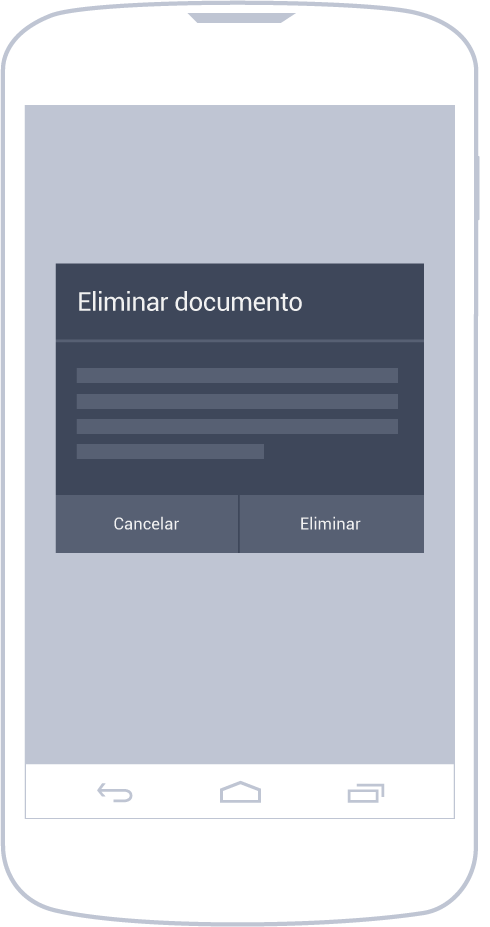
\includegraphics[height=6cm]{img/patron-dialogo-01.png}
\end{figure}
\end{columns}
\end{frame}

%------------------------------------------------

\begin{frame}
\frametitle{Cuadro de Diálogos}

\begin{columns}[c] % The "c" option specifies centered vertical alignment while the "t" option is used for top vertical alignment

\column{.5\textwidth} % Left column and width
\begin{figure}[H]
  \centering
  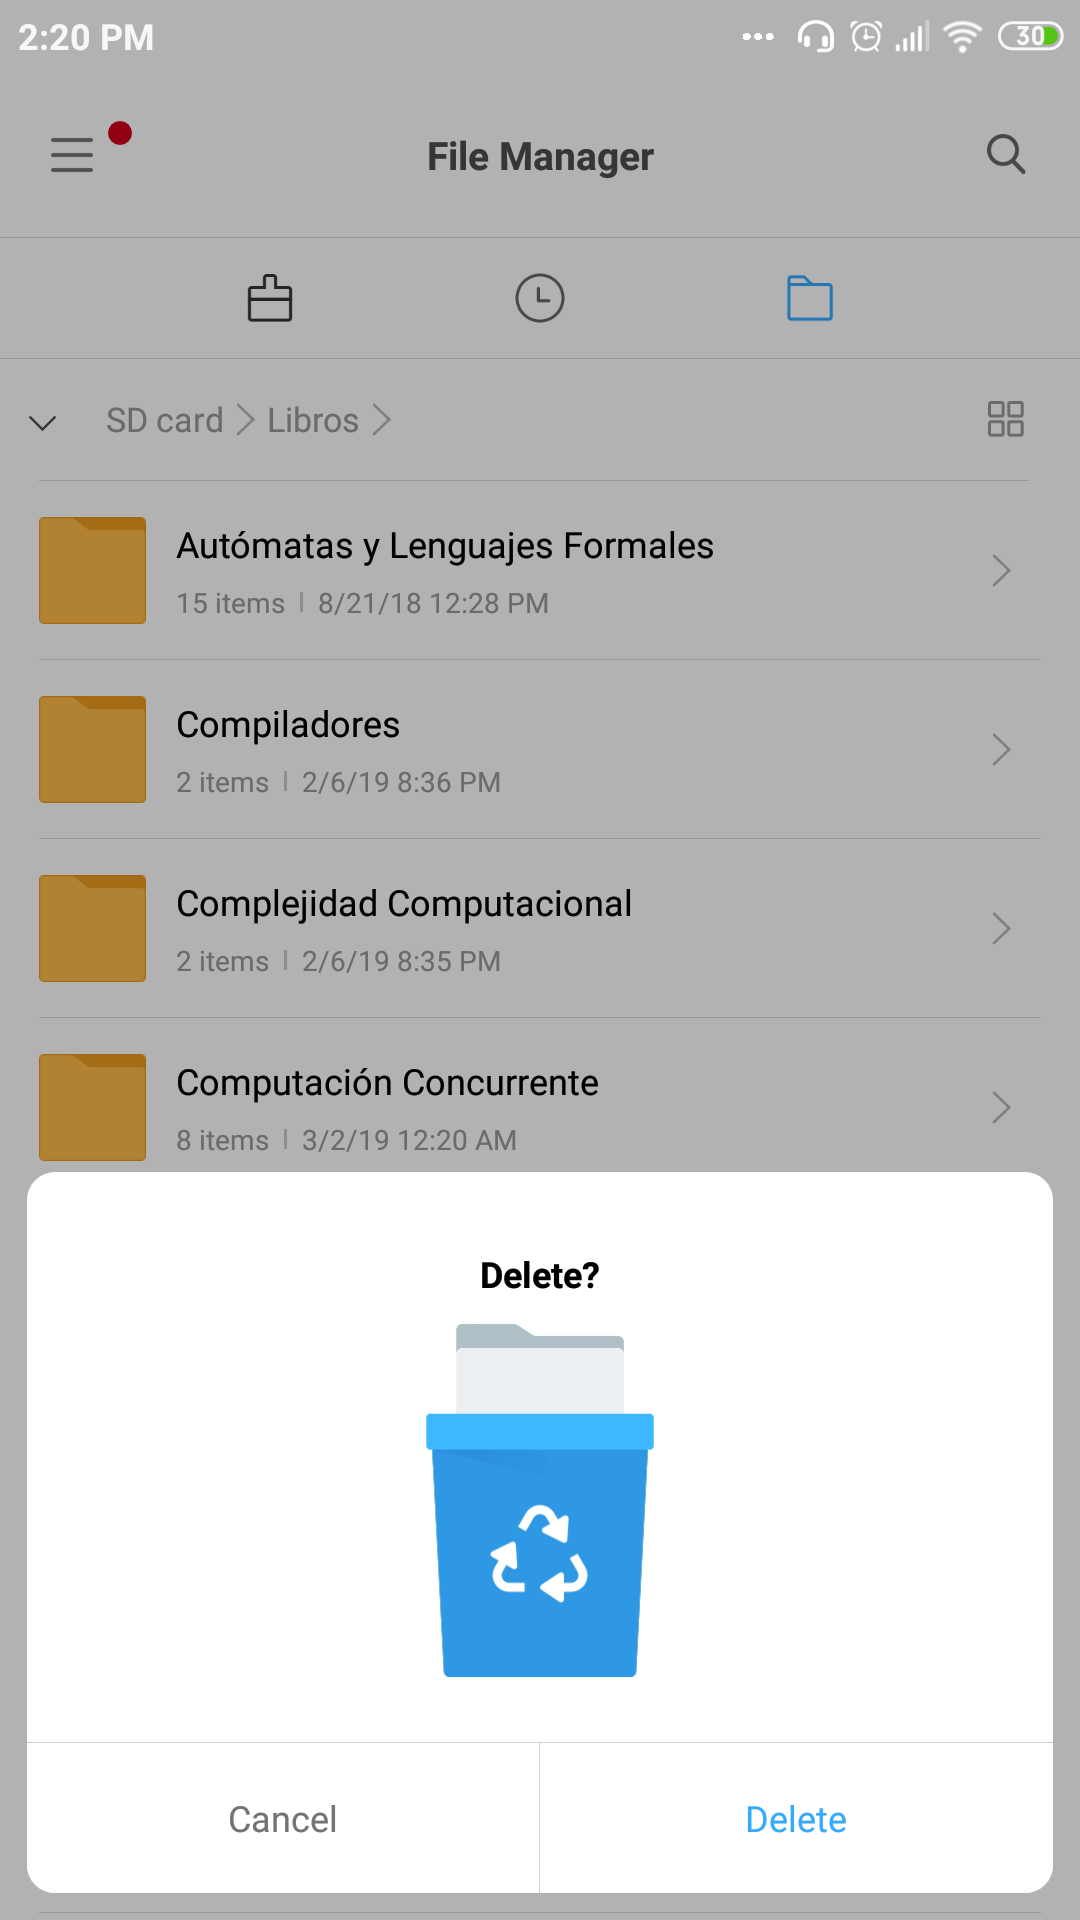
\includegraphics[height=6cm]{img/file-explorer-01.png}
\end{figure}

\column{.5\textwidth} % Right column and width
\begin{figure}[H]
  \centering
  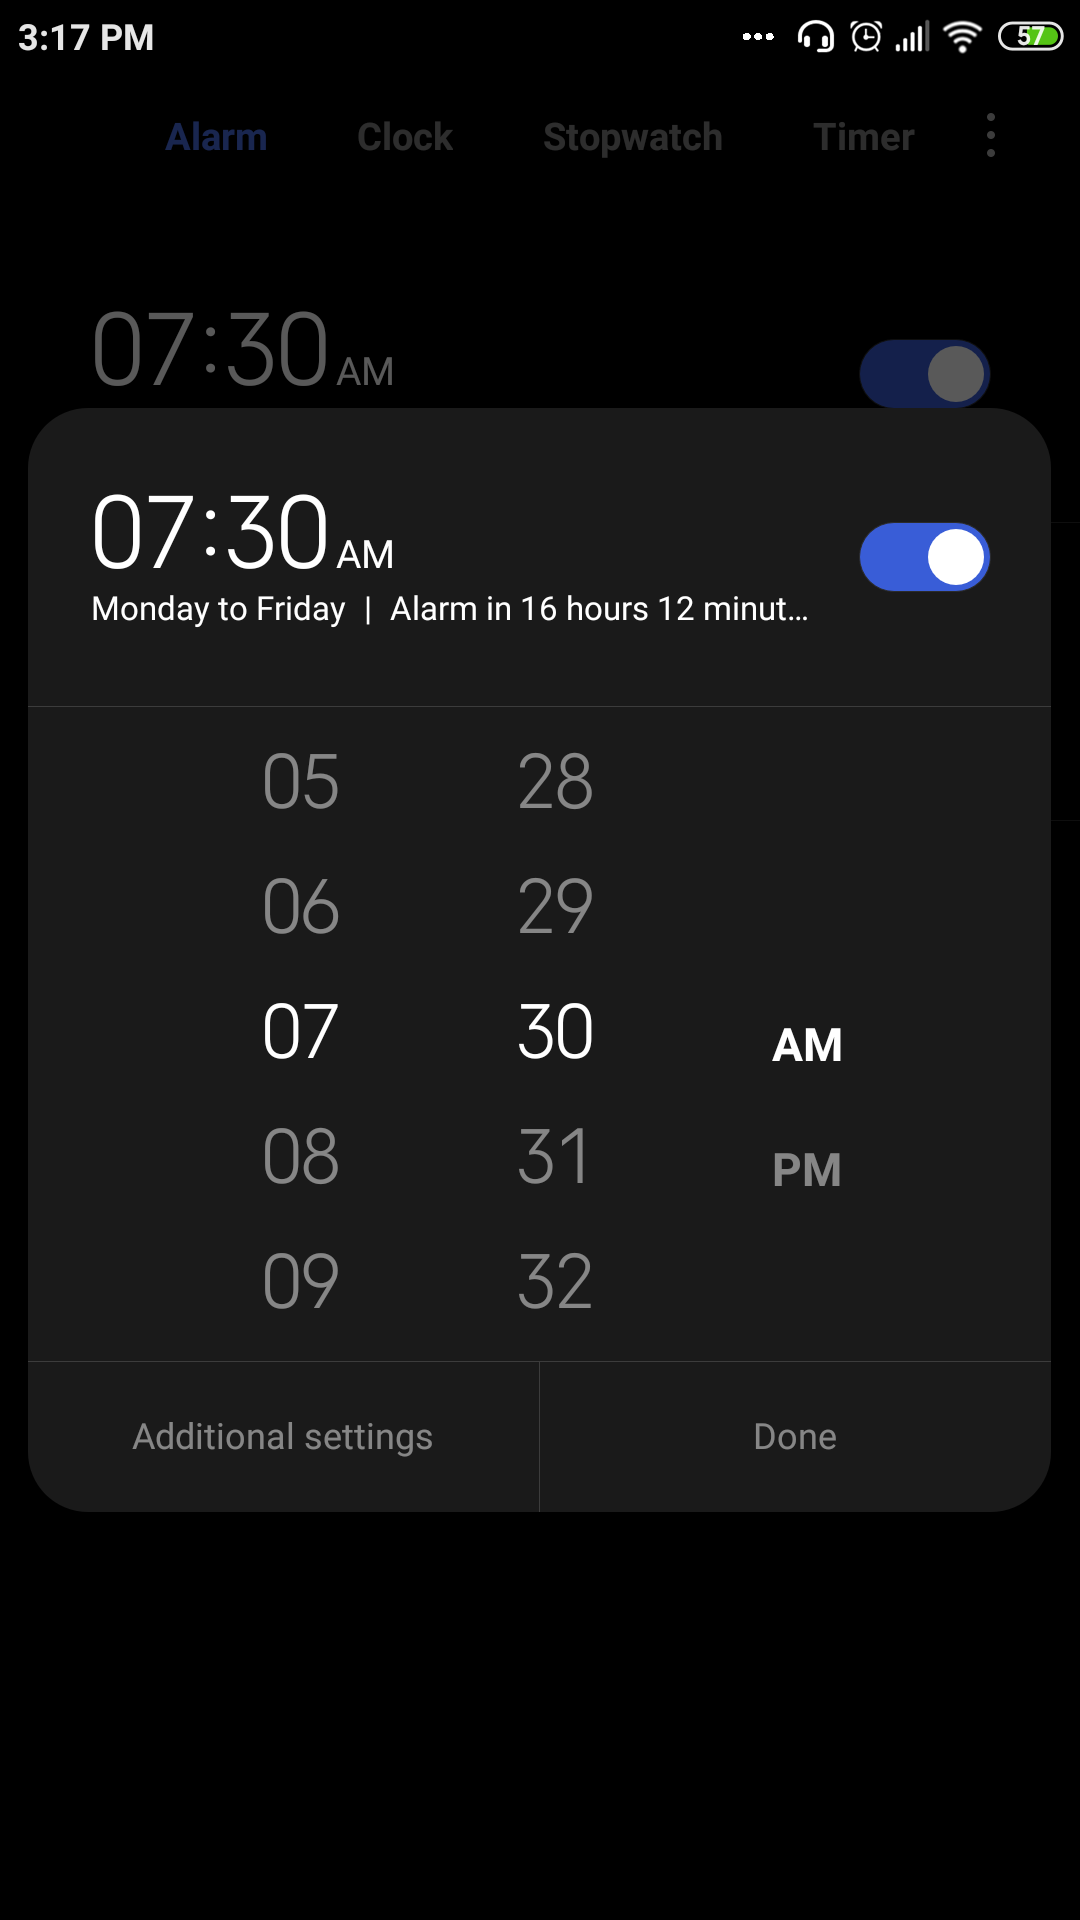
\includegraphics[height=6cm]{img/alarm-02.png}
\end{figure}

\end{columns}
\end{frame}

%------------------------------------------------

\begin{frame}
\frametitle{Cuadro de Diálogos}

\begin{columns}[c] % The "c" option specifies centered vertical alignment while the "t" option is used for top vertical alignment

\column{.5\textwidth} % Left column and width
\begin{block}{iOS}
\justify
Se ubica en el centro de la pantalla, la mayoría de las veces con uno o dos botones en la zona inferior. En caso de tener más de dos botones, se muestran apilados uno sobre otro. Estos diálogos suelen ser tan simples que solo tienen un título, a veces acompañado de una corta descripción.
\end{block}

\column{.5\textwidth} % Right column and width
\begin{figure}[H]
  \centering
  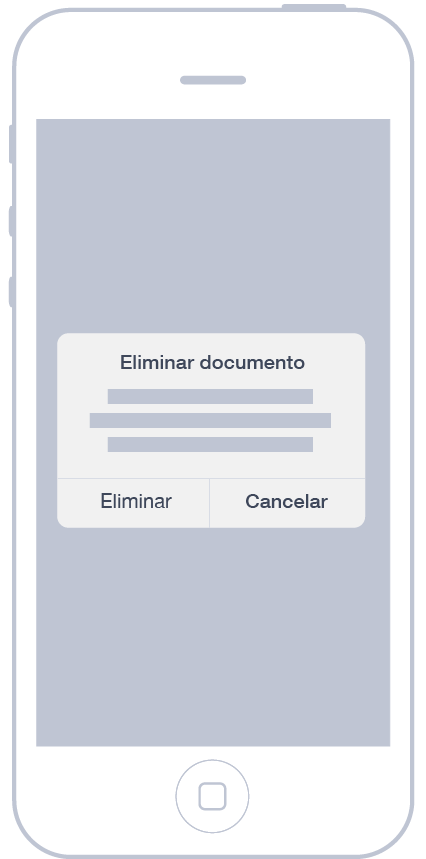
\includegraphics[height=6cm]{img/patron-dialogo-02.png}
\end{figure}
\end{columns}
\end{frame}

%------------------------------------------------

\begin{frame}
\frametitle{Cuadro de Diálogos}

\begin{columns}[c] % The "c" option specifies centered vertical alignment while the "t" option is used for top vertical alignment

\column{.5\textwidth} % Left column and width
\begin{figure}[H]
  \centering
  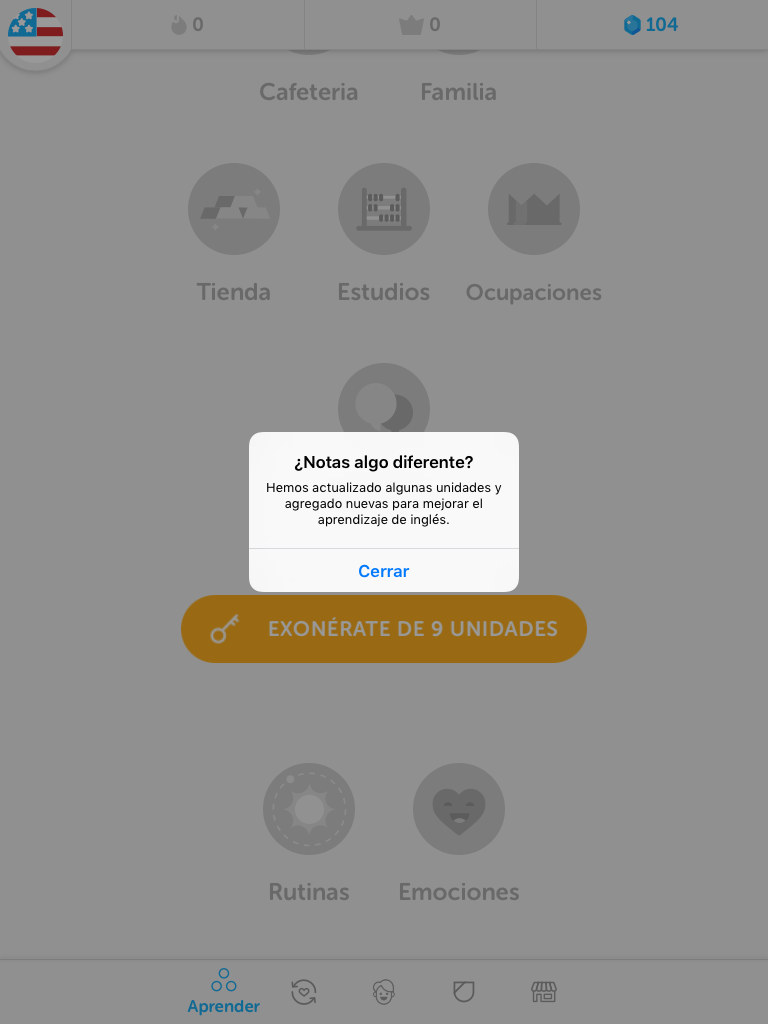
\includegraphics[height=6cm]{img/duolingo-01.PNG}
\end{figure}

\column{.5\textwidth} % Right column and width
\begin{figure}[H]
  \centering
  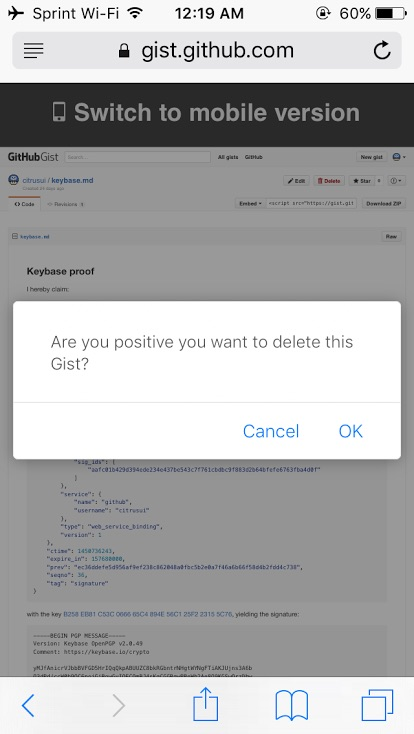
\includegraphics[height=6cm]{img/safari-01.jpeg}
\end{figure}

\end{columns}
\end{frame}

%------------------------------------------------

\begin{frame}
\frametitle{Cuadro de Diálogos}

\begin{columns}[c] % The "c" option specifies centered vertical alignment while the "t" option is used for top vertical alignment

\column{.5\textwidth} % Left column and width
\begin{block}{Windows Phone}
\justify
Los cuadros de diálogo se colocan en la zona superior y pueden ocupar una porción o —\textit{en casos excepcionales}— toda la pantalla.
\end{block}

\column{.5\textwidth} % Right column and width
\begin{figure}[H]
  \centering
  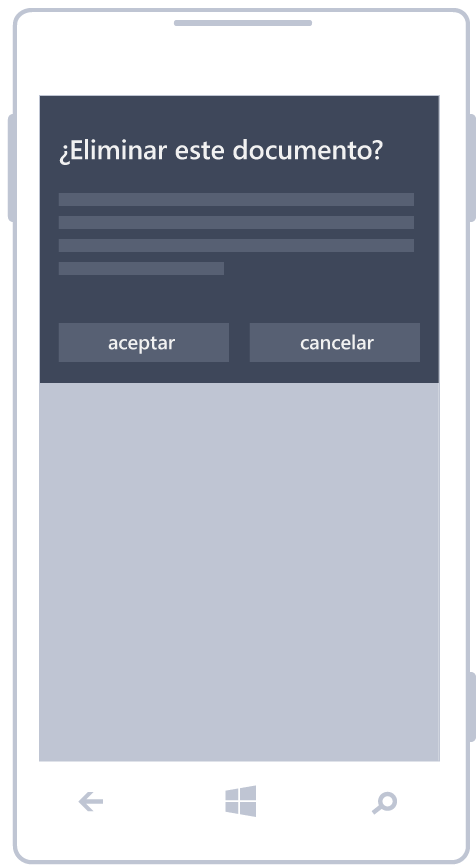
\includegraphics[height=6cm]{img/patron-dialogo-03.png}
\end{figure}
\end{columns}
\end{frame}

%------------------------------------------------

\begin{frame}
\frametitle{Notificaciones Dentro de la Aplicación}

\begin{block}{En resumen:}
\justify
Cuesiones como: ¿Qué está haciendo la \textit{app}? ¿Cómo saber que la acción ha funcionado? ¿Ya terminó o hay que hacer algo más?, seguramente pasan por la cabeza de un usuario cuando no tiene ninguna confirmación visual de que la acción que acaba de realizar.
\end{block}

\begin{figure}[H]
  \centering
  
\includegraphics[height=3.5cm]{img/bell.jpg}
\end{figure}
\end{frame}

%------------------------------------------------

\begin{frame}
\frametitle{Notificaciones Dentro de la Aplicación}

\begin{columns}[c] % The "c" option specifies centered vertical alignment while the "t" option is used for top vertical alignment

\column{.5\textwidth} % Left column and width
\begin{block}{Android}
\justify
Consiste en una «\texttt{toast}», esta notificación aparece por un corto período de tiempo, con un texto —\textit{generalmente de una sola línea}— que le da \textit{feedback} al usuario, por ejemplo, mientras la \textit{app} está guardando un cambio. Al tratarse de un tipo de aviso que puede no ser percibido por el usuario, se usa para comunicar mensajes que no tienen una importancia crítica.
\end{block}

\column{.5\textwidth} % Right column and width
\begin{figure}[H]
  \centering
  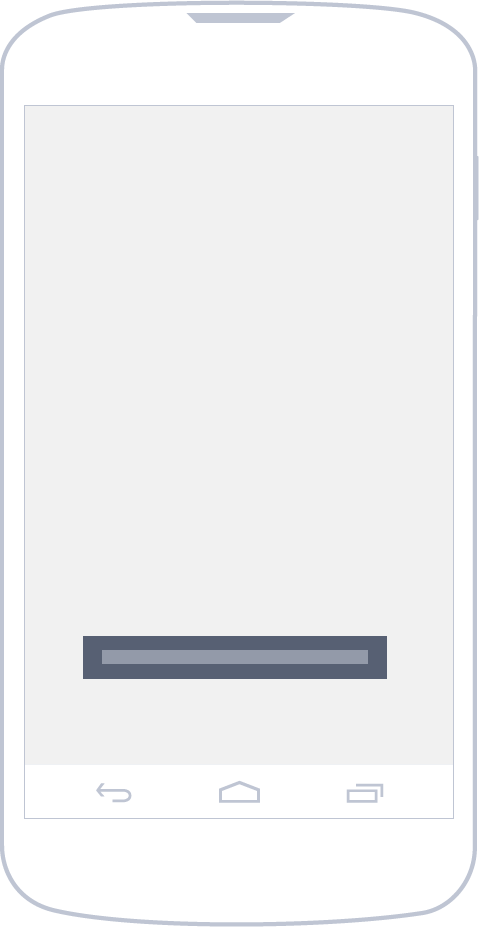
\includegraphics[height=6cm]{img/patron-notificaciones-01.png}
\end{figure}
\end{columns}
\end{frame}

%------------------------------------------------

\begin{frame}
\frametitle{Notificaciones Dentro de la App}

\begin{columns}[c] % The "c" option specifies centered vertical alignment while the "t" option is used for top vertical alignment

\column{.5\textwidth} % Left column and width
\begin{figure}[H]
  \centering
  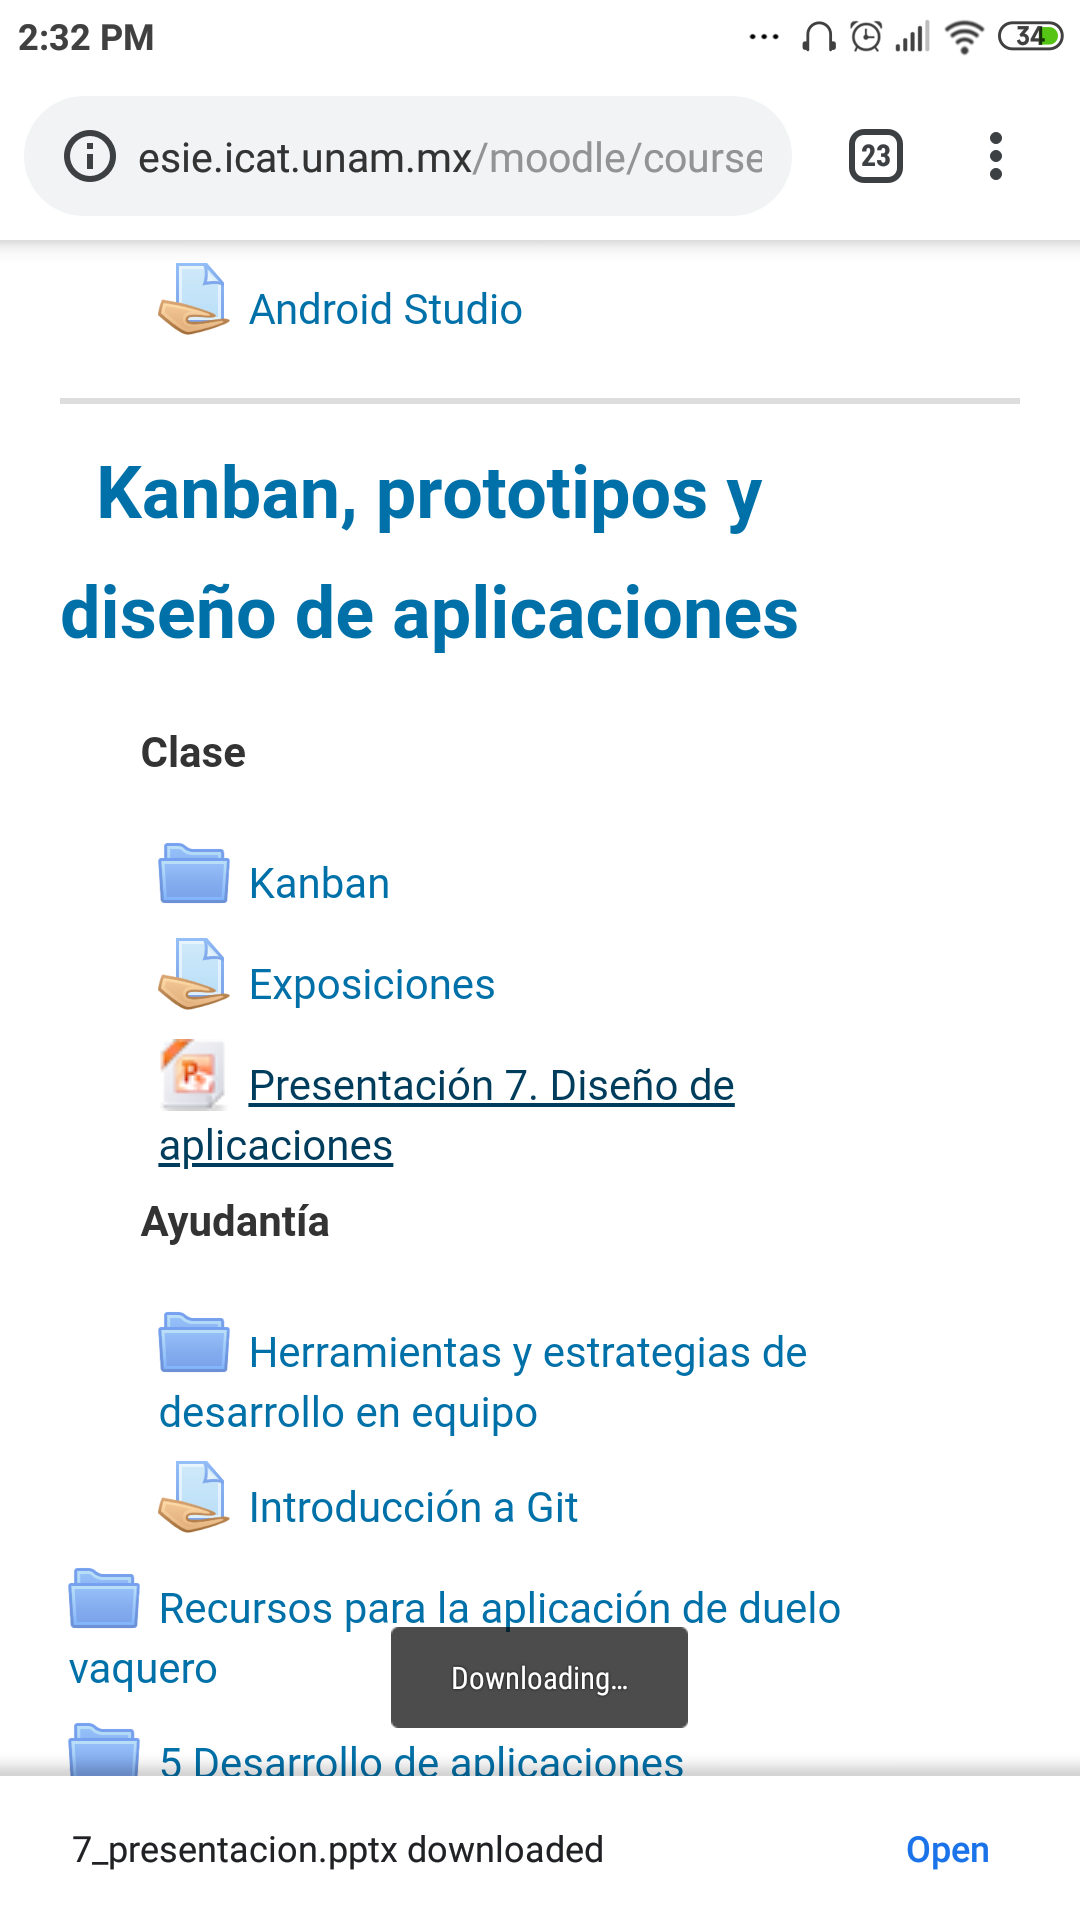
\includegraphics[height=6cm]{img/firefox-01.png}
\end{figure}

\column{.5\textwidth} % Right column and width
\begin{figure}[H]
  \centering
  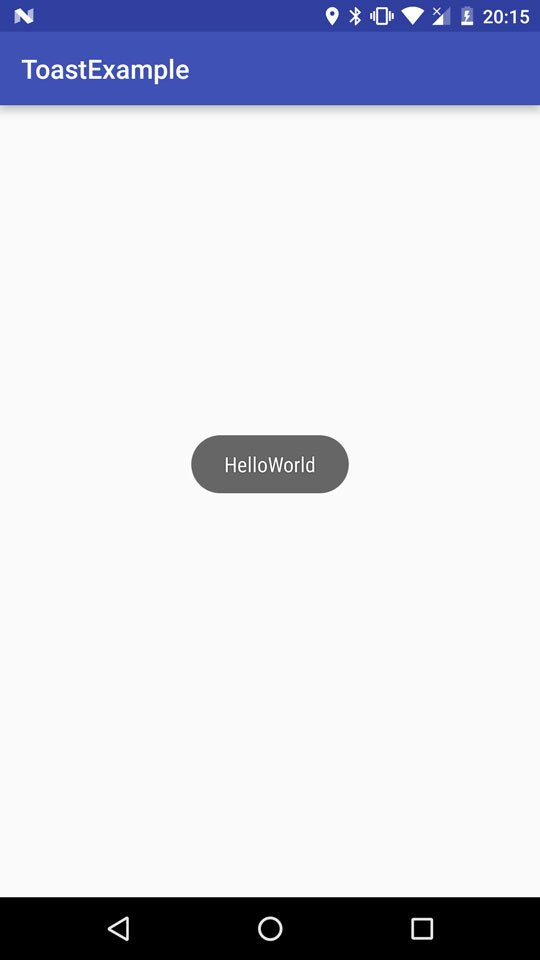
\includegraphics[height=6cm]{img/toast-01.jpg}
\end{figure}

\end{columns}
\end{frame}

%------------------------------------------------

\begin{frame}
\frametitle{Notificaciones Dentro de la Aplicación}

\begin{columns}[c] % The "c" option specifies centered vertical alignment while the "t" option is used for top vertical alignment

\column{.5\textwidth} % Left column and width
\begin{block}{iOS}
\justify
No existe una solución concreta similar a la propuesta de Android, por lo que las notificaciones dentro de la app quedan a cargo del diseñador, por ejemplo, usando librerías externas.
\end{block}

\column{.5\textwidth} % Right column and width
\begin{figure}[H]
  \centering
  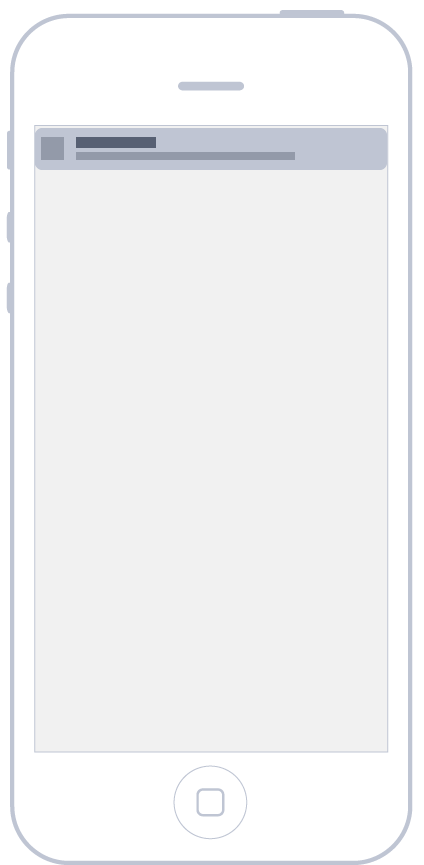
\includegraphics[height=6cm]{img/patron-notificaciones-02.png}
\end{figure}
\end{columns}
\end{frame}

%------------------------------------------------

\begin{frame}
\frametitle{Notificaciones Dentro de la Aplicación}

\begin{columns}[c] % The "c" option specifies centered vertical alignment while the "t" option is used for top vertical alignment

\column{.5\textwidth} % Left column and width
\begin{figure}[H]
  \centering
  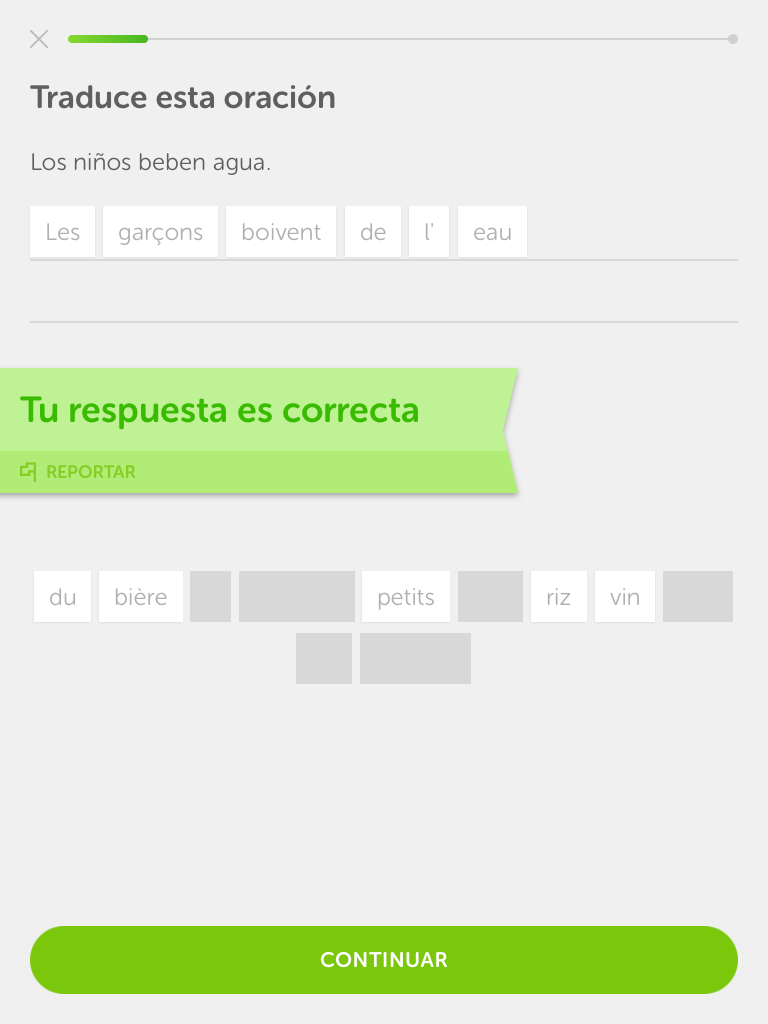
\includegraphics[height=6cm]{img/notification-01.PNG}
\end{figure}

\column{.5\textwidth} % Right column and width
\begin{figure}[H]
  \centering
  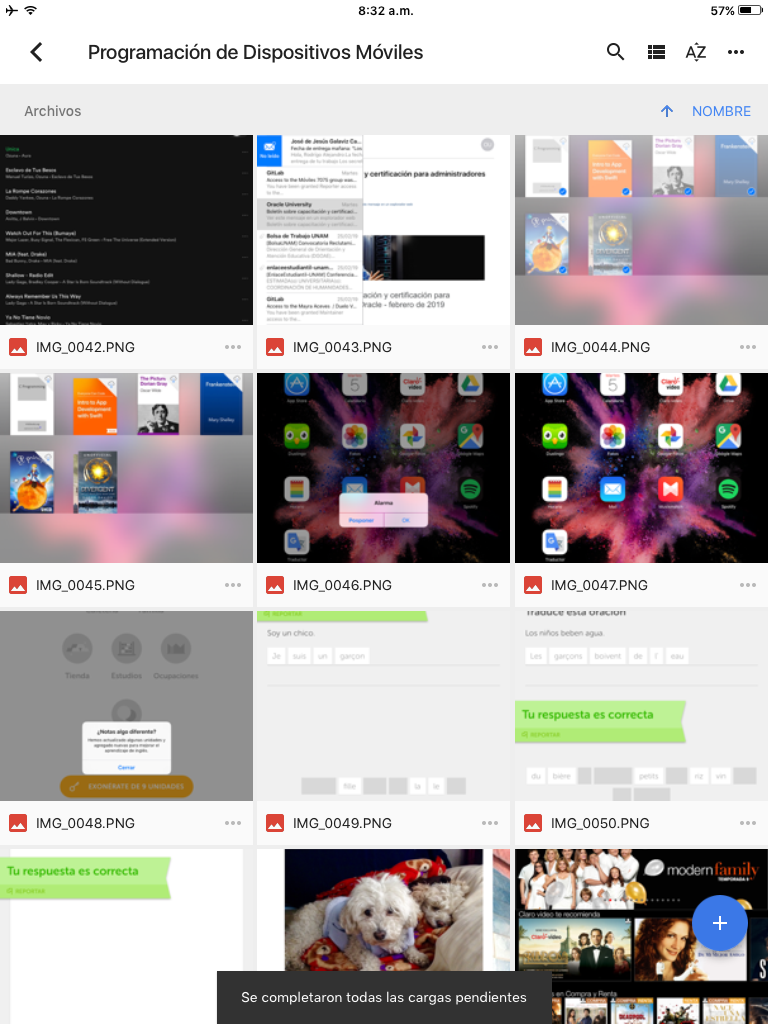
\includegraphics[height=6cm]{img/notification-02.PNG}
\end{figure}

\end{columns}
\end{frame}

%------------------------------------------------

\begin{frame}
\frametitle{Notificaciones Dentro de la Aplicación}

\begin{columns}[c] % The "c" option specifies centered vertical alignment while the "t" option is used for top vertical alignment

\column{.5\textwidth} % Left column and width
\begin{block}{Windows Phone}
\justify
No existe una solución concreta similar a la propuesta de Android, por lo que las notificaciones dentro de la app quedan a cargo del diseñador, por ejemplo, usando librerías externas.
\end{block}

\column{.5\textwidth} % Right column and width
\begin{figure}[H]
  \centering
  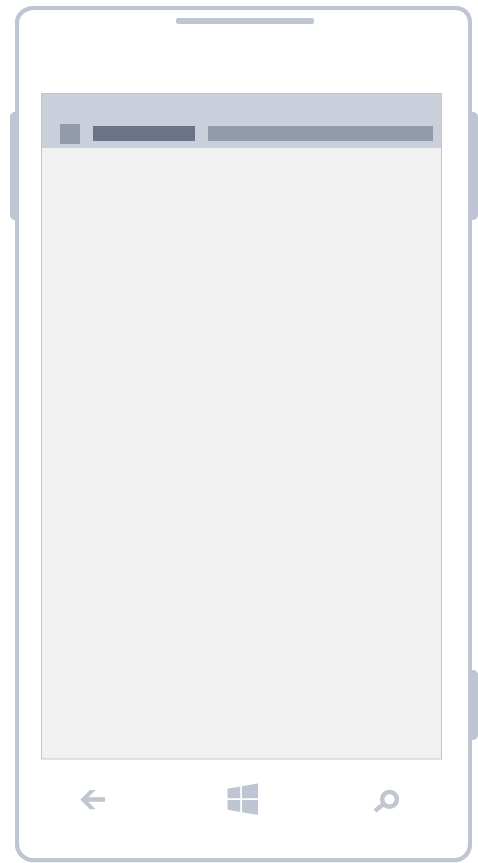
\includegraphics[height=6cm]{img/patron-notificaciones-03.png}
\end{figure}
\end{columns}
\end{frame}

%------------------------------------------------
\section{Actividades}
%------------------------------------------------
\subsection{Relacionar patrones móviles de diferentes sistemas operativos}
%------------------------------------------------

\begin{frame}
\frametitle{Preguntas}

\begin{enumerate}
    \item ¿En qué sistema operativo se implementan las «\texttt{toast}» que consisten en una pequeña «\texttt{pastilla}» en negro que se ubica en la zona inferior de la pantalla y por encima de cualquier otro elemento de la interfaz? \vspace{0.5cm}
    \item ¿En qué parte de la pantalla se encuentra comúnmente la barra de búsqueda en los sistemas operativos de los móviles? \vspace{0.5cm}
    \item ¿En los cuadros de diálogos de Android las solicitudes pueden ser más complejas que botones de «\texttt{aceptar}» o «\texttt{cancelar}»?
\end{enumerate}
\end{frame}

%------------------------------------------------

\begin{frame}
\frametitle{Post-it!}

\begin{figure}[H]
  \centering
  \includegraphics[height=6cm]{img/post-its.png}
\end{figure}
\end{frame}

%------------------------------------------------
\section{Referencias}
%------------------------------------------------
\subsection{El final}
%------------------------------------------------

\begin{frame}
\frametitle{Referencias}
\footnotesize{
\begin{thebibliography}{99} % Beamer does not support BibTeX so references must be inserted manually as below
\bibitem[]{p1} App Design Book, \emph{Capítulo 7, Interacción y patrones}.
\newblock (Consultado el 26 de febrero, 2019).
\newblock \url{http://appdesignbook.com/es/contenidos/patrones-interaccion-moviles/}

\bibitem[]{} Designing Interfaces, \emph{2nd edition}. \newblock (Consultado el 26 de febrero, 2019).
\newblock \url{http://esie.icat.unam.mx/moodle/pluginfile.php/110/mod_resource/content/1/Designing.Interfaces.2nd.Edition.PDF.pdf}

\bibitem[]{} Wikipedia, \emph{Patrón de Diseño}.
\newblock (Consultado el 26 de febrero, 2019)..
\newblock \url{https://es.wikipedia.org/wiki/Patr\%C3\%B3n_de_dise\%C3\%B1o}

\end{thebibliography}
}
\end{frame}

%------------------------------------------------

\begin{frame}
\Huge{\centerline{¡Gracias por su atención!}}

\begin{figure}[H]
  \centering
  \includegraphics[width=8cm]{img/android_kotlin.png}
\end{figure}
\end{frame}

%------------------------------------------------

\end{document}